\chapter{Spatial Audio: Capture \& Reproduction} \label{ch:spat-aud}

\section{Introduction}
%This chapter will be developed with Tamara Smyth.

In this chapter, we will shift the focus from spatial music to spatial audio. We will begin by drawing a line from the inception of recorded sound to the latest developments in 3D audio, including advancements in cross-talk cancellation (XTC), WFS, and ambisonics. In this chapter, we are concerned with the variety of ways that sound engineers can use spatial audio technologies to record and reproduce spatial music. We will also touch upon some of the technical complications of this work that might prove problematic for engineers (ie. insufficient memory, speaker count, hardware requirements, etc.).

In particular, this chapter will focus on the main technology this author is concerned with: ambisonics. One of the major benefits of ambisonics is the \textit{isotropic}\footnote{Identical in all directions; invariant concerning direction. In an ambisonic context, this means the sound field can be reproduced in whatever sound system is available.} nature of the design, which makes it more flexible than surround sound standards such as 5.1. Ambisonics has a long-established tradition in the spatial audio community and as such, a myriad of open source tools have already been developed for its usage. These tools make it more accessible in many ways that \textit{object-based audio} (OBA) ecosystems, most of which are proprietary and closed-source. With the proliferation of systems for binaural rendering, ambisonics has resurfaced as a reliable method for spatial audio reproduction, especially in XR environments.

In addition to listing and demystifying the different spatial audio technologies available today for playback, we will suggest engineering approaches for the capture of spatial sound, which can be leveraged towards asynchronous or synchronous dissemination. In particular we will focus on FOSS as in the rest of this text. These spatial audio recordings can later be used in immersive environments such as the ones described in Chapter \ref{ch:xr-mus}. In contrast to Chapter \ref{ch:spat-mus}, which outlines technologies which are better suited for real-time performances with musicians, in this chapter we will highlight tools for creating \textit{fixed-media} works, such as videos or movies.

\section{History of Spatial Audio Capture \& Reproduction}

\subsection{Audio Pioneers} \label{subsec:audio_pioneers}

The invention of the telephone, in 1876, by Alexander Graham Bell\footnote{Scottish-born inventor, scientist, and engineer.} \cite{grosvenor2016alexander} can be considered the genesis of all \textit{spatial audio} technologies. The transmission principles it used where what later inspired the development of the phonograph\footnote{Colloquially known as a record player, the phonograph, or gramophone, was also used to record sound signals. Today, most people know it exclusively as a playback system.}, one of the first known recording devices, invented by Thomas Edison\footnote{Edison (February 11, 1847 – October 18, 1931) was an American inventor and businessman who has been described as America's greatest inventor.} in 1877 \cite{gitelman1999scripts}. This subsequently galvanized a whole new generation of engineers who developed more sophisticated methods for sound capture and reproduction. 

\begin{figure}[ht]%force figure here, top, 
\centering
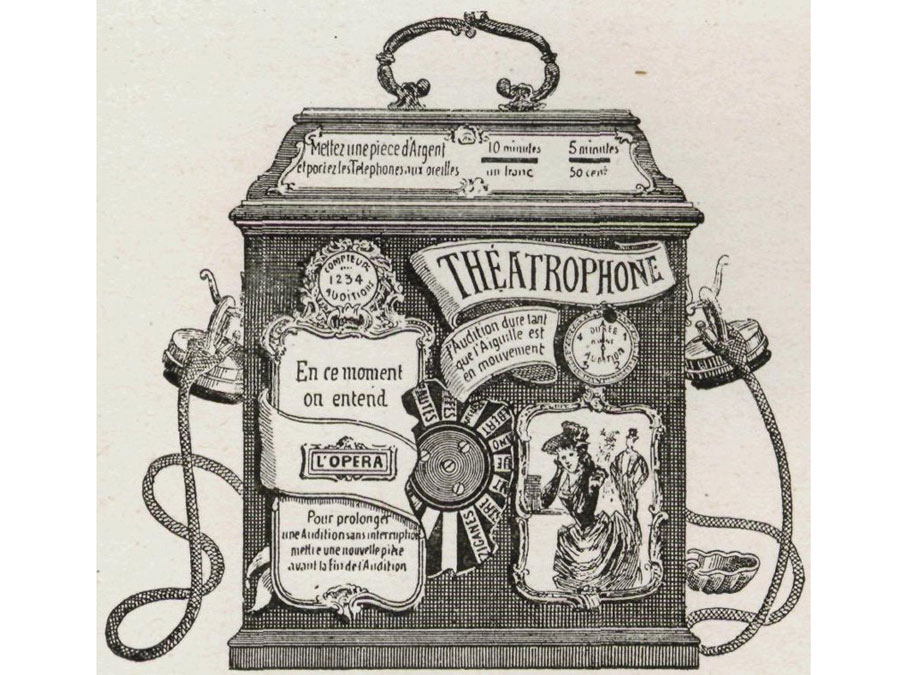
\includegraphics[width=0.7\textwidth]{img/theatrophone.jpeg} 
%\captionsetup{justification=centering}
\caption{Théâtrophone \cite{theatrophonepic}}
\label{fig:theatrophone}
\end{figure}

A few years after the invention of the phonograph, Clément Ader\footnote{Ader (2 April 1841 – 3 May 1925) was a French inventor and engineer from Toulouse.}, best known for his work in aviation systems, would present the \textit{théâtrophone}: a "system of telephonic transmission where listeners received a separate channel for each ear, enabling \textit{stereophonic} perception of actors on a set". Ader presented his prototype at the Paris Exhibition for Electricity in 1881 \cite{malham19953}. Figure \ref{fig:theatrophone} shows a picture of the device; in the image, one can see the two receivers which would be placed at the listeners ears for stereophonic playback. The writing on the image also shows the cost for the audience member, which was 10 minutes for one franc, or 5 minutes, for 50 cents. This device should not be confused with the additive synthesizer entitled \textit{Telharmonium} (1896) by Cahill, described in Chapter \ref{ch:spat-mus}. While both devices were used for long-distance music transmission, the théâtrophone was based on transmission of microphone signals, as opposed to synthesis of musical tones via electric means. 

Decades would pass before any new major developments in the field would occur, but eventually, in the 1920's, Harvey Fletcher\footnote{Fletcher (September 11, 1884 – July 23, 1981) was an American physicist. He is known as the "father of stereophonic sound".}, from Bell Telephone Laboratories\footnote{Bell labs has an important place in computer music history. It is where Max Mathews wrote the first computer music language, MUSIC-N.}, developed one of the first binaural recording systems. This system used the anatomy of the head to naturally embed spatial attributes of sound to recordings \cite{harvey1927binaural}. It would not be, however, until 1933, at the Chicago Century of Progress Exhibition, that binaural recordings would first be introduced to the public. 

Fletcher is believed to also be responsible for the first public demonstration of stereophonic sound, which took place in 1934 in New York City. Bell Telephone Laboratories, along with Fletcher, is also accredited for, in the 20's, being the first American institutions to research what is known today as \textit{Wave Field Synthesis} (WFS): a system which captures a "wall of sound", using an array of microphones, and then consequently plays it back - using an array of speakers \cite{fletcher1942hearing}\footnote{While Fletcher would be one of the first to describe the idea of WFS in 1942, it would not be until 1988 that Berkhout would propose the mathematics involved in WFS to transform a single sound source into a wall of sound using a synthesis approach.}.

Later, in 1933, Fletcher also demonstrated the possibilities of long-distance multi-channel sound transmission. In a collaboration with English conductor Leopold Stokowski\footnote{Leopold (18 April 1882 – 13 September 1977) was a British conductor of mixed Polish and Irish descent.}, considered one of the first stereo control-board operators\cite{mcginn1983stokowski}, Harvey and other Bell Lab engineers put together a system which transmitted the sound of an orchestra in Philadelphia via three microphones placed on stage to three corresponding loudspeakers in Washington DC's Constitution Hall. Bell Labs and Stokowski would go on to collaborate on numerous events in the 40's. 

Around the same time Alan Blumlein, an American engineer, was working on a much simpler yet powerful spatial audio technique: high-fidelity stereophony. Blumlein's most important contribution to the field of spatial audio is perhaps his \textit{Mid/Side} (MS) encoding technique, which he patented in 1931 \cite{billingsley1987simulated}. This technique provided audio engineers with stereo width control by mixing microphone signals with different patterns, polarities, and gains. Blumlein's design consisted of taking the output of a \textit{figure-8} microphone and summing it with an \textit{omni-directional} microphone. A second copy of the figure-8 microphone would be phase inverted. The result were two cardioid like patterns with the same orientation as the stereo-speaker arrangement. Figure \ref{fig:ms_stereo} shows the general set-up for the MS stereo recording technique\footnote{Note the panning on the two copies of the figure-8 microphone.}. The technique was later expanded by Michael Gerzon\footnote{British mathematician and sound engineer.}, in the 1970's, to develop the first \textit{First Order Ambisonic}\footnote{Also known as a tetrahedral or sound-field microphone.} (FOA) microphone, which constitutes one of the first multi-channel recording systems.  

\begin{figure}[h!]%force figure here, top, strict
\centering
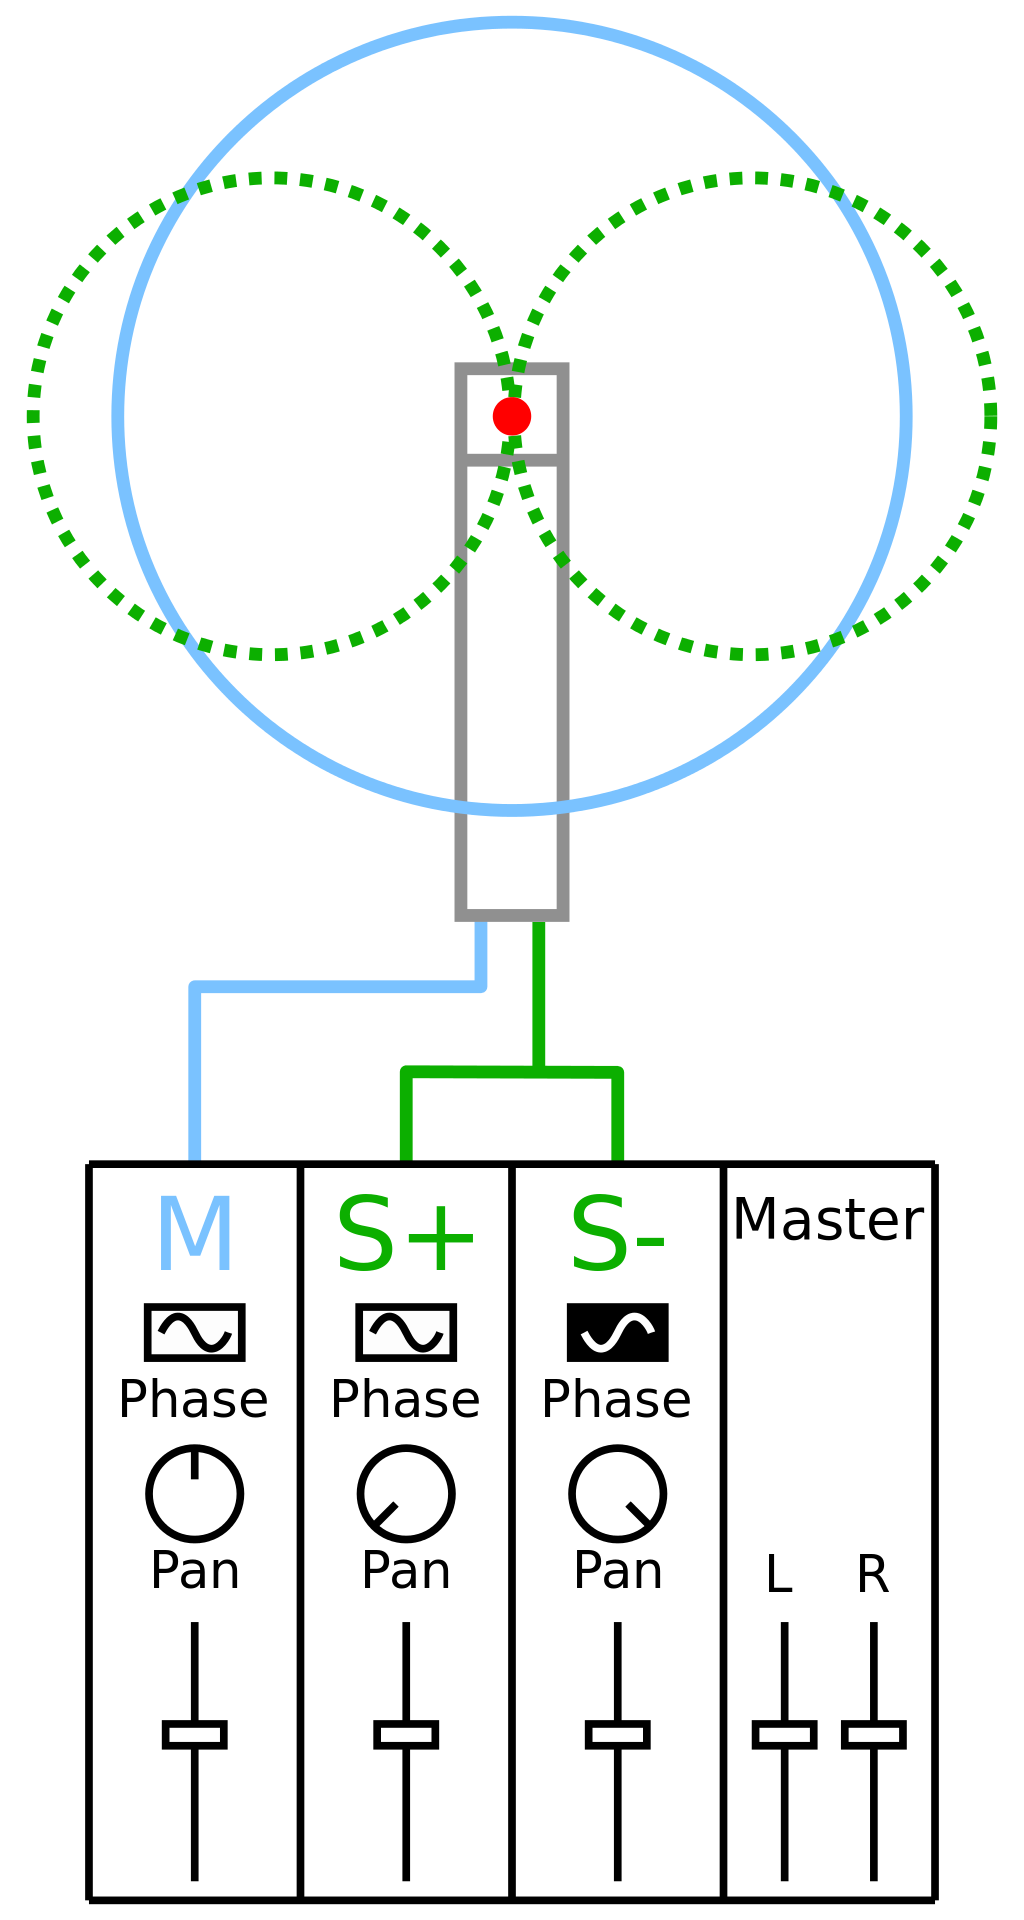
\includegraphics[width=0.35\textwidth]{img/ms_stereo.svg.png} 
%\captionsetup{justification=centering}
\label{fig:ms_stereo}
\caption{Mid-Side Stereo \cite{ms_stereo_pic}}
\end{figure}

In 1940, a few years after Blumlein's patent, Leopold Stokowski, RCA, and Disney, released the film \textit{Fantasia}, which featured a system called \textit{Fantasound}. The control system they designed allowed audio tracks to be panned to any of 10 loudspeakers \cite{klapholz1991fantasia}. Moderate improvements to sound quality and storage capacity were achieved from 1940 to 1970. 

In the 1970's, a different and significantly more obscure technology was being developed: \textit{quadraphonic sound}. Quadraphonic research is believed to have begun at the \textit{Acoustic Research Corporation} by Robert Berkovitz \cite{davis2003history}. The idea was to use two rear channels to produce the ambience of the recording, and two front channels for direct sound - the most important being dialogue. Unfortunately, due to a number of: financial, engineering, and marketing issues, the system never gained much popularity. This technology did however inspire other breakthroughs.

The development of encoding and decoding schemes for quadraphonic sound would eventually pique the interest of British mathematician Michael Gerzon\footnote{Gerzon (4 December 1945 – 6 May 1996) is probably best known for his work on Ambisonics and audio systems. He was also interested in free improvisation in music.}. Michael would, in 1969, present to the public a new audio capture method inspired by Alan Blumlein, and the rise in interest in quadraphonics. Gerzon proposed, provocatively, the use of a tetrahedral array for audio capture in which the four signals could be encoded into three coincident\footnote{Coincident meaning placed close together.} figure-8 microphones. This system, Gerzon believed, could optimize the use of the four speakers by providing listeners with not only horizontal information, but also vertical sound. Unfortunately, the system suffered from a considerably small ideal listening area or \textit{sweet spot}\footnote{Higher Order Ambisonics (HOA), developed much later, in the 90's, has been shown to increase the size of the sweet spot.}, a fact which detracted many sound system engineers who were primarily concerned with immersive audio for large film theatres.

Around the same time that Gerzon was presenting his FOA microphone to the world, Tom Horall, of what today is known as Acentech\footnote{\href{https://www.acentech.com/}{Acentech website link.} (Accessed: Mar 5, 2021)} decided to attempt to recreate the acoustics of the famous Boston Symphony Hall using an acoustical model. The system used tape delay techniques to achieve believable spatial sound. Using a dozen loudspeakers Horall was able to convince the listeners that they were actually being transported to the iconic hall. The system would later be commercialized in 1988 and become known as the Pioneer DSP-3000 \cite{davis2003history}. 

Many other developments followed suit from the 80's to today. Perhaps the most popular of these being the 5.1 surround sound system. Today, there is an ongoing battle regarding the future of spatial audio. Companies are consistently looking for scalable and reliable solutions to improve sound quality for patrons. Unfortunately, many of these systems have suffered from their distinctly complicated set-up process or high costs. The quest for: simple, high-fidelity, three-dimensional sound, continues. 

%\subsection{Stereo Techniques}
\subsection{Binaural Microphones}

\textit{Binaural audio} and \textit{multi-channel stereophony} are the two most common spatial audio technologies. \textit{Binaural audio} has become increasingly popular for \textit{virtual reality} (VR) while \textit{multi-channel stereophony} can be found in home entertainment systems as well as automotive sound systems. Stereo, however, is still the prevailing reproduction format, which is why binaural microphones have gotten some interest as a means of "static" spatial audio reproduction. Others have written about \textit{transaural} sound systems, which reproduce \textit{binaural audio} over stereo sound systems. \textit{Transaural} reproduction is a niche system that has been gaining more interest in the community. The underlying technology, however, seems to remain limited to audiophiles and a number of select engineers working on it.

In contrast to other spatial audio recording methods, which rely on large arrays of microphones, binaural recordings only use two microphones to encode spatial information into a stereo recording. Binaural recordings are either captured using a \textit{dummy-head}, a mannequin head with microphones inside its ears, or with \textit{in-ear} microphones placed inside a person's ear canals, to capture what they would normally listen to. They can also be synthesized using \textit{virtual surround sound} software applications, a subject we will cover in more detail later. By playing back these binaural recordings using headphones, ear-buds, or with stereo speakers - using \textit{cross-talk cancellation} (XTC) filters\footnote{XTC is also referred to as \textit{transaural reproduction} in the literature.} - a person can sense a sonic space around them as it originally occurred. 

Unfortunately, some issues arise from this method. Firstly, people's heads and ears differ in size and shape, a fact which distorts the recordings ever so slightly breaking the illusion that one has been transported from their current location to the new auditory scene. Secondly, when the listener hears back the recording, they will be striped of \textit{rotational} control. In other words, when they turn their heads, the sound will remain fixed in the same perspective as the original recording.

As a result, the illusion of immersion will be lost. The lack of \textit{auditory parallax}\footnote{Parallax is the effect whereby the position or direction of an object appears to differ when viewed from different positions.} creates localization errors and \textit{internalization} of sound sources. Internalization refers to the perception that sound sources originate from inside our heads, rather from external sources: this is the only logical conclusion since moving our heads does not change the sound-field. Figure \ref{fig:dummy-head} shows a "dummy head": a binaural microphone with two capsules placed inside the modeled \textit{pinnae}, mimicking the behavior of the human cochlea\footnote{The biological structure in our inner ear where frequency analysis is performed.}. The pinnae in these systems tends to be manufactured using a soft plastic such as silicone to mimic the absorption of human cartilage on sound.

\begin{figure}[ht!]%force figure here, top, strict
\centering
\includegraphics[width=0.7\textwidth]{img/dummy-head.jpg} 
%\captionsetup{justification=centering}
\caption{Dummy Head \cite{FileGeor45online}}
% This file is licensed under the Creative Commons Attribution-Share Alike 2.0 Generic license.
\label{fig:dummy-head}
\end{figure}

\textit{Binaural recordings} are not a particularly good representation of the desired sound-field resulting from a \textit{spatial music} work, however, they are crucial for the development of binaural synthesis systems, which ultimately can convey a more realistic representation of the musical work. Often, it becomes impractical to use a real human for \textit{Head Related Transfer Function} (HRTF)\footnote{Filters which simulate the effect of the human head on sound.} sampling, since the process can take a long time, and, human movements during acoustic sampling can lead to errors in the data-set. In this context, an anthropomorphic average of a human head, is better suited for the sampling task. Alternatively, the binaural impulse responses can be synthesized using acoustic models. Algazi et al. \cite{algazi2002use}, for example, describes a head-and-torso model, or "snowman" model, to efficiently implement HRTF approximations towards real-time spatialization. 

\begin{equation} \label{eq:conv-hrir}
\begin{array}{l}
x_{L}(n)=\sum_{p=1}^{P} x_{p}(n) * h_{L, \theta_{p}, \phi_{p}}(n) \\
x_{R}(n)=\sum_{p=1}^{P} x_{p}(n) * h_{R, \theta_{p}, \phi_{p}}(n)
\end{array}
\end{equation}

Hacihabiboglu et al. \cite{hacihabiboglu2017perceptual} provide a simple equation for the \textit{auralization} of a virtual signal via convolution with two HRIRs\footnote{Head Related Inpulse Responses, or HRTFs taken in diffuse-field conditions.}. This is equivalent to the process of filtering the source $x_p$ with a filter whose frequency response would be identical to the Fast Fourier Transform (FFT) of $h_{R, \theta_{p}, \phi_{p}}$ and $h_{L, \theta_{p}, \phi_{p}}$ respectively. The topic of \textit{binaural synthesis} will be discussed further in later sections, as it is a primary area of interest in modern 3D audio research.

Binaural microphones are still very much in production today, and several moderate improvements have been made to them over the years. However, for the most part, these devices remain the same as they were 30 years ago. One interesting project, elucidated by Johansson's \cite{johansson2019vr} paper, is the idea of "dynamic HRTFs" data-sets, which would require the development of a motorized \textit{Head and Torso Simulator} (HATS). This would allow various neck angles to be simulated. To our knowledge, all the HATS have a fixed neck angle, but in the real world, sometimes we move our heads independently of our bodies to localize sound. Johansson suggests that future HRTF sets should include separate shoulder and head acoustic information.

\subsection{Sound-field Microphones}

\textit{First Order Ambisonic} (FOA) microphones were developed initially in the 70's by Michael Gerzon, from Oxford's department of Mathematics, and Peter Fellgett, from the University of Reading \cite{elen1991whatever}, under the supervision of the National Research Development Corporation (NRDC) in England. Gerzon and Fellgett were indubitably inspired by Alan Blumlein's work in the field of stereophony. Blumlein was the pioneer of various audio technologies, chief among them a sum-and-difference matrix system which was capable of creating high quality stereo recordings. The \textit{Mid-Side} recording technique simply derives two cardioid patterns from the combination of one omni-directional microphone, closely positioned with a figure-8 microphone. Gerzon and Felgett had the notion that a 3D sound system could be created by adding 2 additional figure-8 microphones, each representing a different 3D axis (X, Y, Z). 

However, instead of using 3 figure-8 microphones, Gerzon and Fellgett went in the opposite direction: they figured out a way to derive these three microphones from four cardioid microphones, mounted on the faces of a tetrahedron. Consider Figure \ref{fig:foa-patt-n-mic}: on the left, we can see the polar pattern of the FOA mic from a birds-eye view. On the right, we see a drawing of the actual microphone\footnote{Created by Yigal Kamel from "The Cooper Union for the Advancement of Science and Art".}. As we can see from this top view, three orthogonal figure-8 microphones can be derived from the sum and difference of these different microphones. For example, to derive the front-back microphone we sum the front capsules and subtract the back capsules. The sides will cancel out and we will be left with a figure-8 response. 

\begin{figure}
\centering
\begin{subfigure}{.5\textwidth}
  \centering
  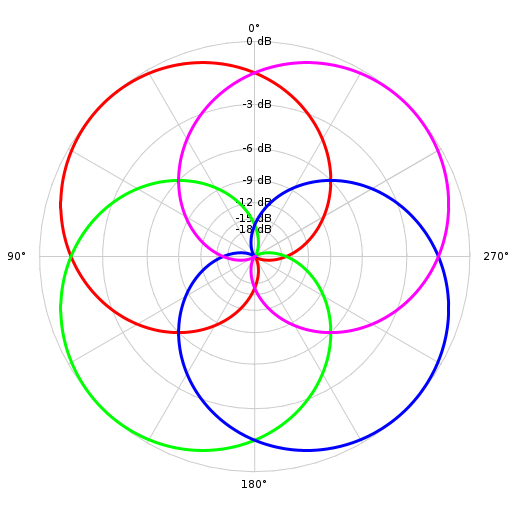
\includegraphics[width=.6\linewidth]{img/foa-pattern.png}
  \caption{FOA Patterns (Top View) \cite{FileNaiv77online}}
  \label{fig:foa-patt}
\end{subfigure}%
\begin{subfigure}{.5\textwidth}
  \centering
  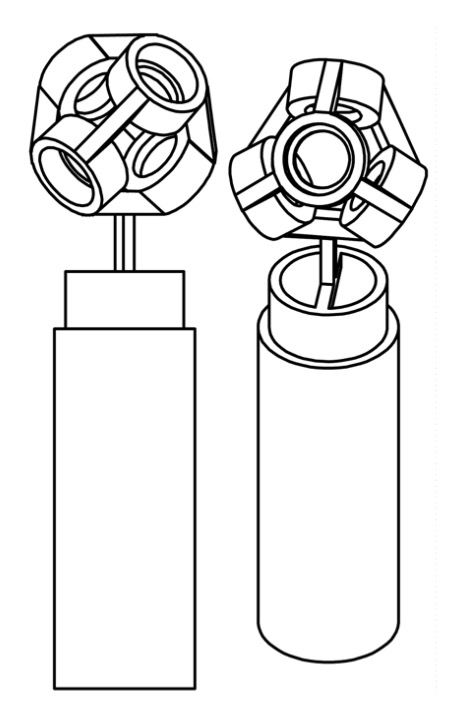
\includegraphics[width=.6\linewidth]{img/yigal-kamel.JPG}
  \caption{SolidWorks Drawing FOA Microphone}
  \label{fig:yigal-kamel}
\end{subfigure}
\caption{FOA Polar Patterns (Top View) and CAD Drawing of FOA Mic}
\label{fig:foa-patt-n-mic}
\end{figure}

In addition to the three orthogonal figure-8 microphone signals, an additional omni-direction channel, often denoted with the letter W, can be encoded by summing the four cardioid capsules. Once these four signals are recorded, they can be \textit{decoded} into any number of different reproduction systems. For example, the combination of signals can be used to yield a stereo representation with good mid/side separation. For example, the UHJ system, also known as "C-format", was an ambisonic system designed to be compatible with mono and stereo media. 

One of the main problems with ambisonics, or any surround sound reproduction system for that matter, is correct speaker placement. As Elen \cite{elen1991whatever} points out:

\begin{quote}
    "Most readers, I am sure, have visited numerous friends who keep their stereo loudspeakers in some very odd places -- one channel behind the sofa and the other on top of the bookcase, for example. It’s hard enough to get people to put two speakers in sensible places for stereo -- what about four for surround sound?"
\end{quote}

\subsubsection{Ordering and Normalization}

Another problem, from the engineering perspective, can be the confusing naming and labeling of capsules, which is crucial to proper encoding. Furthermore, there needs to be harmony between the signal order in the encoder and decoder, otherwise the decoding will not work properly. For example, if an X channel is switched with a Y channel, the source localization will be completely off, and the listener will likely not be satisfied. This problem is only exacerbated in HOA systems, which can contain dozens of ambisonic harmonics. 

An additional consideration is the \textit{normalization} system used in the encoding of the signals. Normalization refers to the practice of weighting the different ambisonic channels such that the vectors will not only be \textit{orthogonal} but also \textit{ortho-normal}. That is, each component of the sound-field will represent the same amount of energy. The normalization should be matched between encoder and decoder, otherwise an excess of a particular signal might be introduced into each of the channels, distorting the balance between direct sound and diffuse sound. 

\todo[inline]{define orthogonal and orthonormal?}

Luckily, today we can rely on certain standards for \textit{ordering} of ambisonic channels and their normalization. Chief among these are the \textit{Furse-Malhalm} (FuMa) ordering scheme and the \textit{ACN} (Ambisonic Channel Number) scheme. For converting between these different "conventions" (including normalization and ordering) Kronlachner \cite{kronlachner2014plug} provides a free DAW-based plug-in. These are useful for example if one's publishing platform\footnote{Ie. Youtube, Vimeo, Facebook.} only supports one ordering style. Table \ref{tab:ambi-ordering} shows these two ordering schemes. 

\todo[inline]{add citation for fuma and acn ordering?}

% http://excel2latex.com/ 
\begin{center}
    \begin{tabular}{ | l | l | l | }
    \hline
	Ambisonic Ordering Conventions (3OA) &  &  \\ \hline
	 & FuMa & ACN \\ \hline
	W & 0 & 0 \\ \hline
	Y & 2 & 1 \\ \hline
	Z & 3 & 2 \\ \hline
	X & 1 & 3 \\ \hline
	V & 8 & 4 \\ \hline
	T & 6 & 5 \\ \hline
	R & 4 & 6 \\ \hline
	S & 5 & 7 \\ \hline
	U & 7 & 8 \\ \hline
	Q & 15 & 9 \\ \hline
	O & 13 & 10 \\ \hline
	M & 11 & 11 \\ \hline
	K & 9 & 12 \\ \hline
	L & 10 & 13 \\ \hline
	N & 12 & 14 \\ \hline
	P & 14 & 15 \\ \hline
    \end{tabular}
    \label{tab:ambi-ordering}
\end{center}

At this point, FuMa, and the \textit{maxN} normalization scheme it used, seem to be mostly unsupported. Developers are instead focusing on the Ambix format which consists of the ACN ordering scheme and \textit{Schmidt semi-normalized} harmonics format (SN3D). We included the FuMa ordering for completeness, but we hope in a few years the ordering scheme will be entirely defunct. These discrepancies in ordering are part of what detracts more developers from working with ambisonics. The following equation shows the SN3D normalization, according to Gorzel's 2019 \cite{gorzel2019efficient} paper on the implementation of Resonance\footnote{Resonance is an open-source Google product for ambisonic manipulation.}. 

\begin{equation}
N_{n}^{|m|}=\sqrt{\left(2-\delta_{m}\right) \frac{(n-|m|) !}{(n+|m|) !}}
\end{equation}

Another normalization standard is the N3D normalization scheme. The N3D normalization standard is defined by the following equation \cite{politis2016jsambisonics}:

\begin{equation}
N_{n}^{|m|}= \sqrt{(2 n+1) \frac{(n-|m|) !}{(n+|m|) !}}
\end{equation}

Where $\delta_m = 1$ for $m$ = 0, and 0 otherwise. In the Ambix specification paper \cite{nachbar2011ambix}, one should note there is a $1/4\pi$ term that is ignored in our formula. Ultimately, if we treat this term as a scalar, since it is independent of \textit{ambisonic order} ($n$), or \textit{ambisonic degree} ($m$), we can see that it can justifiably be omitted.

\subsubsection{Ambisonic Degree and Order}

In mathematics and physics, the order ($m$) and degree ($l$) of spherical harmonics is the opposite of the ambisonic order ($n$) and ambisonic degree ($m$). In other words, the Ambisonic order is the mathematical degree of the spherical harmonic, and the Ambisonic degree is the mathematical order of the spherical harmonic. 

% $m$ = mathematical order = ambisonic degree = $m$, 
% and
% $l$ = mathematical degree = ambisonic order = $n$.

\begin{figure}[ht!]%force figure here, top, strict
\centering
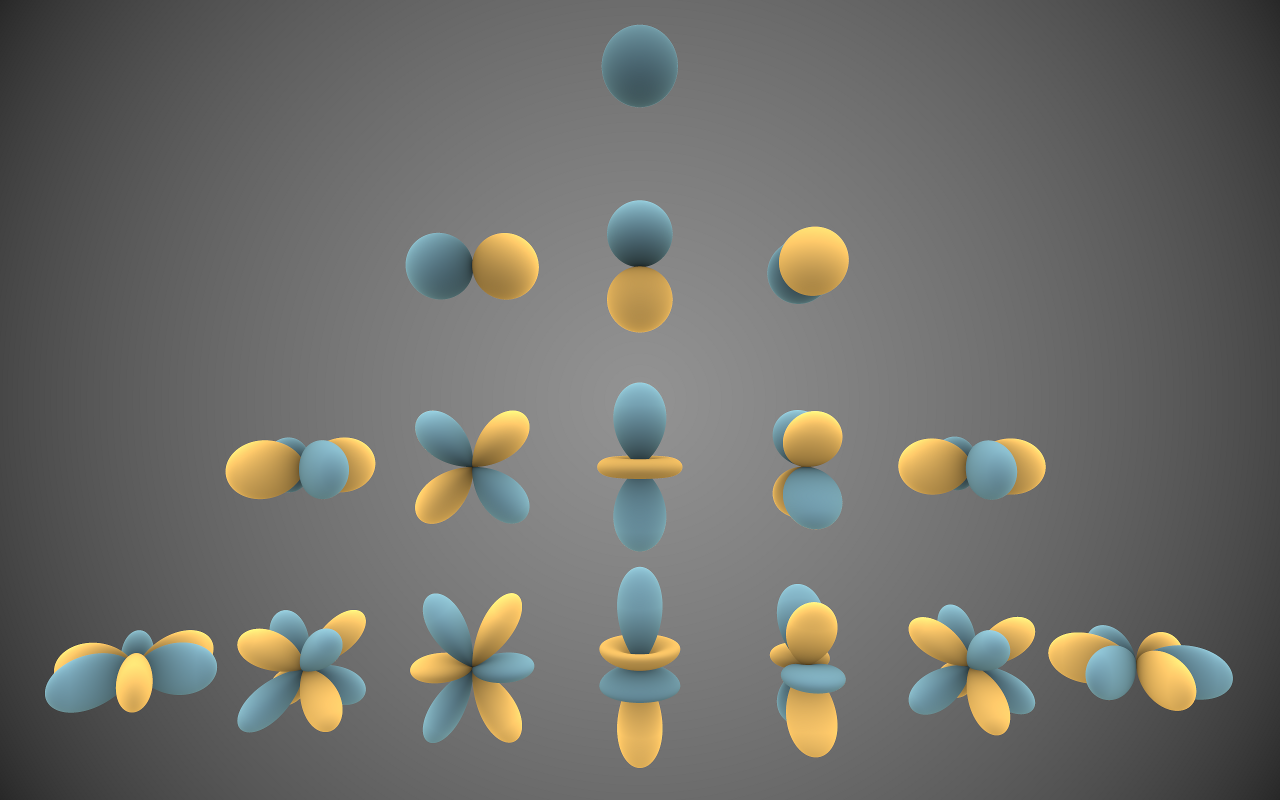
\includegraphics[width=0.6\textwidth]{img/sph-harm.png}
 %cc by-sa 3.0
\caption{Spherical Harmonics \cite{Spherica39online}}
\label{fig:sph-harm}
\end{figure}

Figure \ref{fig:sph-harm} shows a classic representation of spherical harmonics of increasing \textit{degree} ($l$), where the top harmonic has a degree of 0 and the bottom harmonic has a degree of $L$. The \textit{order} ($m$), in the mathematical sense, spans from negative to positive values and includes 0. 

In order to avoid confusion when we refer to ambisonic order, we will always use the term \textit{ambisonic order}. For example, in Figure \ref{fig:sph-harm}, the ambisonic order ($n$) increases from 0 to $N$, where the top harmonic has an ambisonic order of 0 and the bottom harmonic has an ambisonic order of $N$. The ambisonic degree ($m$) spans from negative to positive values and includes 0. 

Another confusing matter is that the 3D coordinate system used is not always the same across all these technologies, especially when we switch over to different spatial audio methods such as VBAP or OBA. For example, in SpatDIF, the azimuth angle increases clockwise and the X, and Y, axes are switched relative to the Ambix convention. 

In this text, when talking about ambisonics, we will use $\phi$ to denote the azimuth angle, increasing in the anti-clockwise direction, and $\theta$ to denote the elevation angle, increasing upwards to 90\textdegree. The x, y, and z axes point front, left and up respectively. The conversion between spherical and Cartesian coordinates is defined as: 

\begin{equation}
\begin{array}{l}
x=\|\vec{r}\| \cos (\phi) \cos (\theta) \\
y=\|\vec{r}\| \sin (\phi) \cos (\theta) \\
z=\|\vec{r}\| \sin (\theta)
\end{array}
\end{equation}

\todo[inline]{define r.}

\begin{figure}[ht!]%force figure here, top, strict
\centering
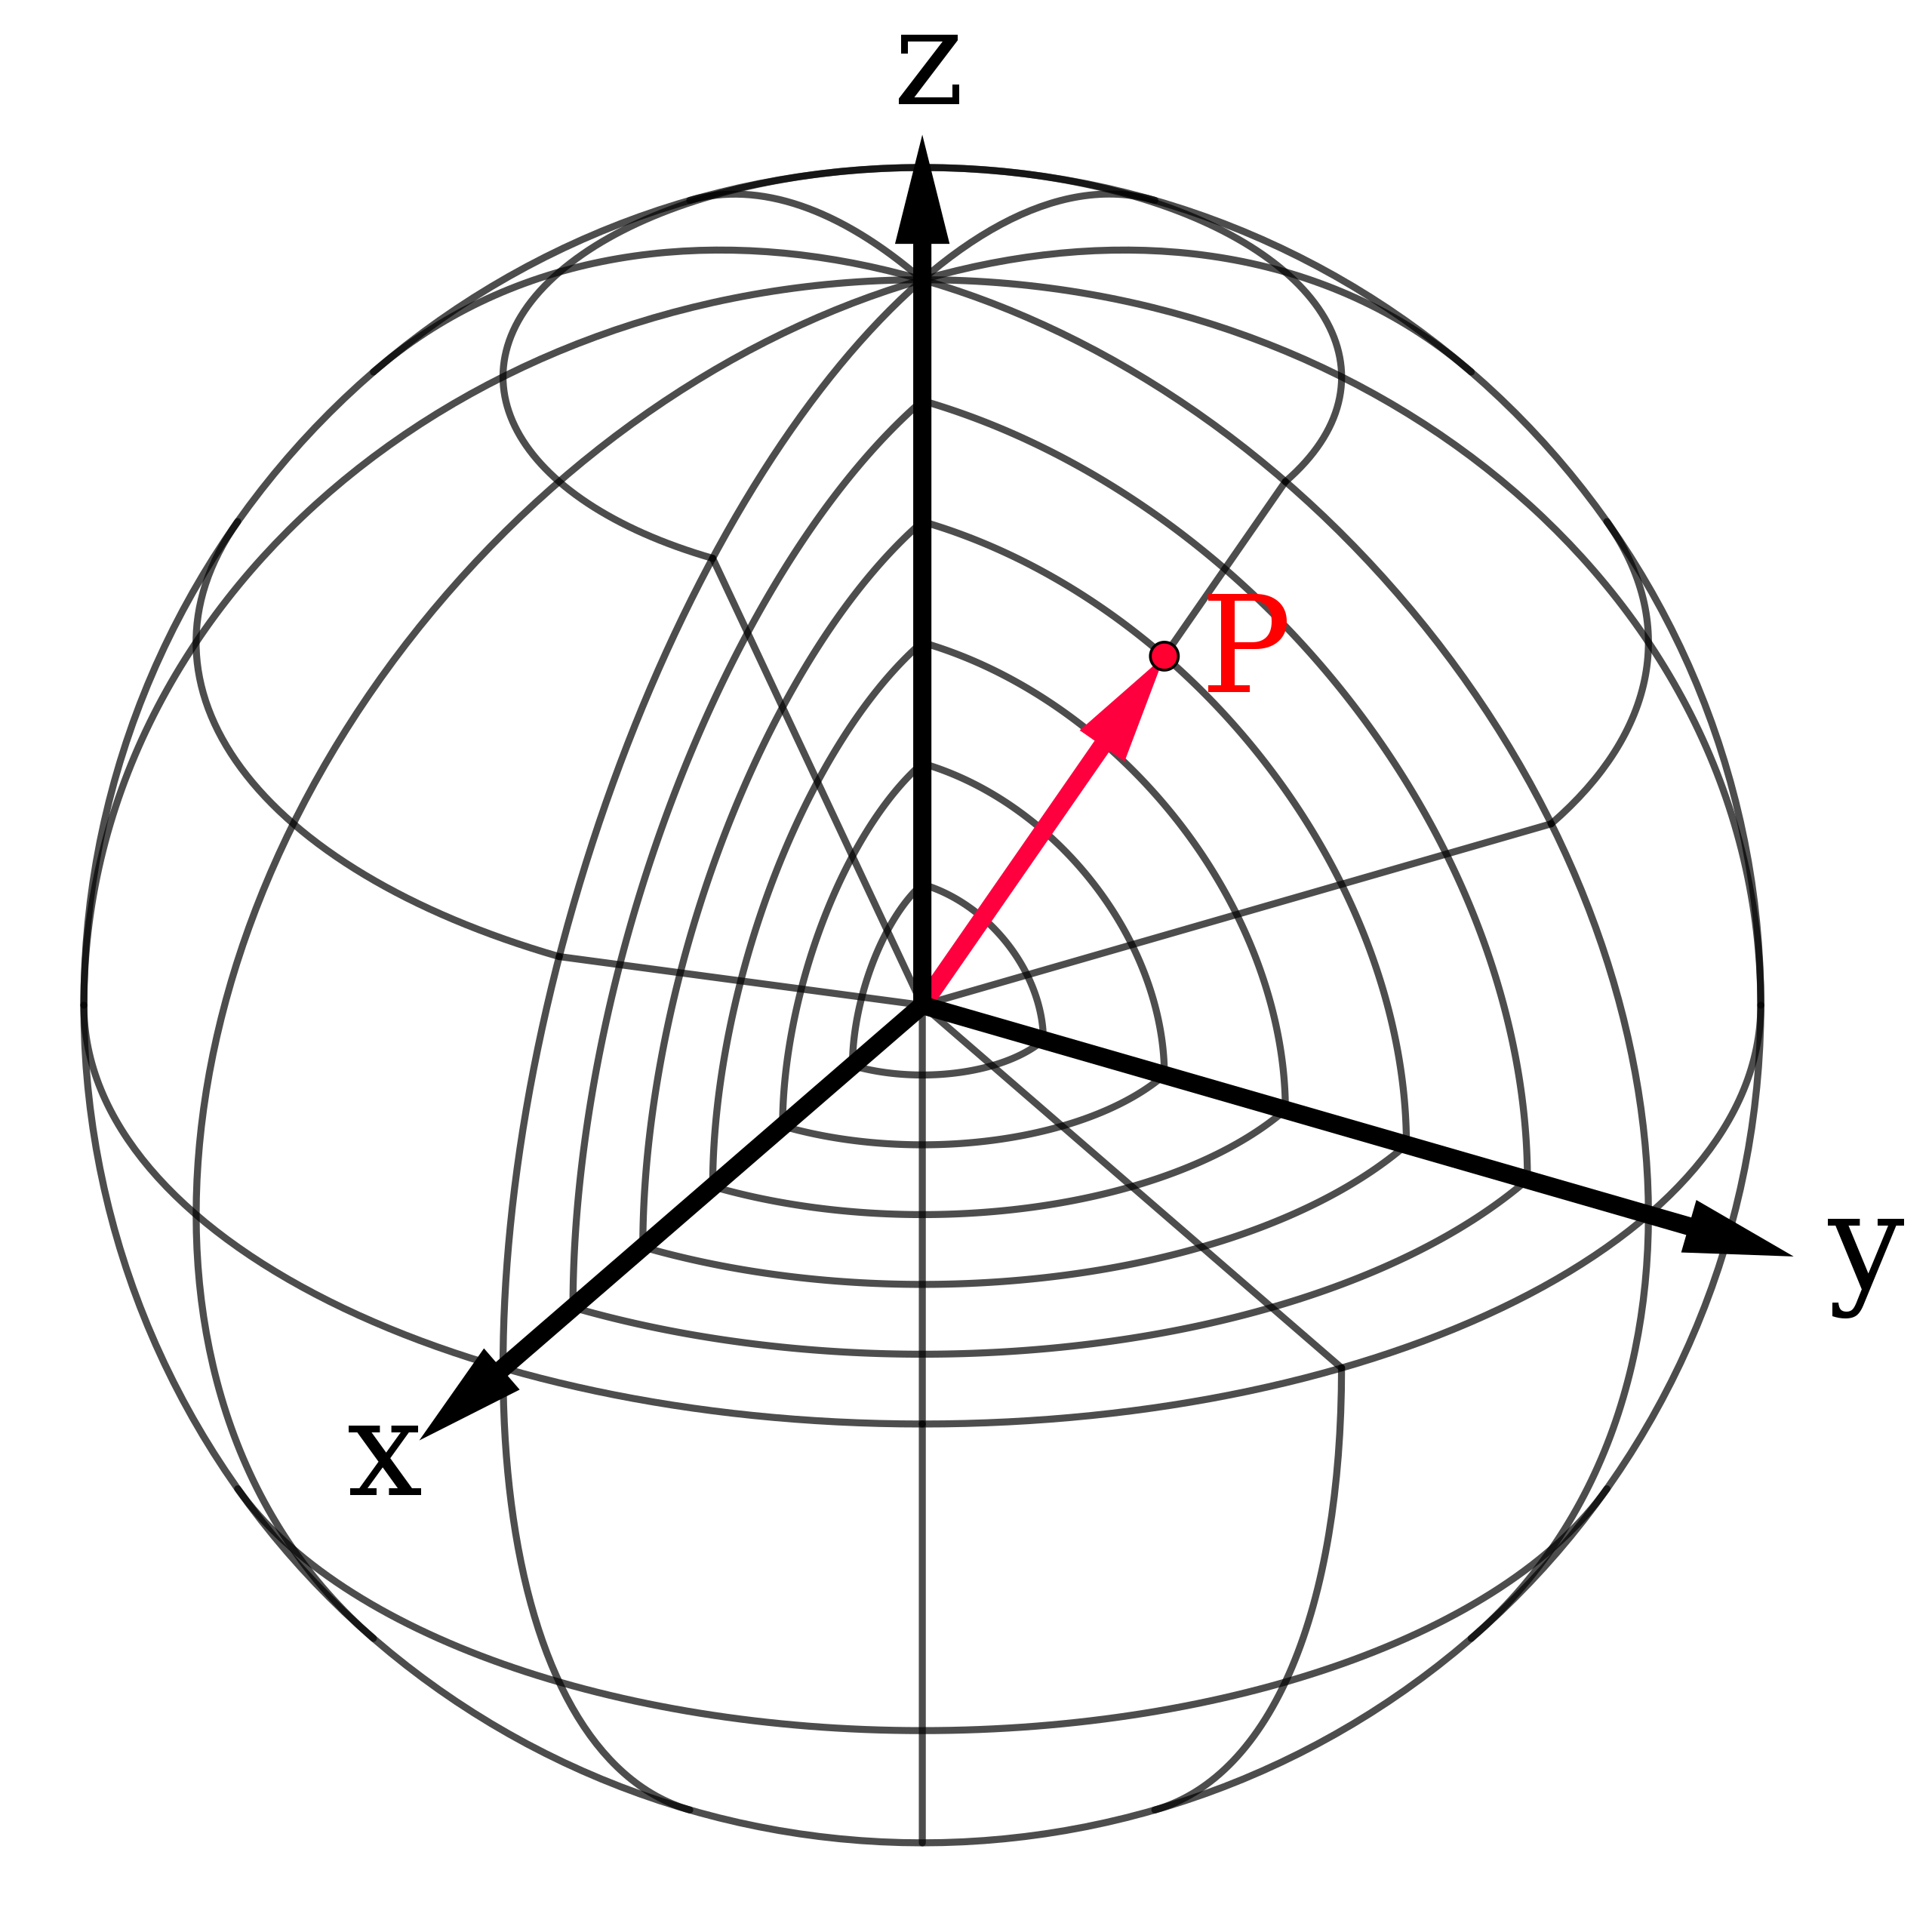
\includegraphics[width=0.5\textwidth]{img/sph-coord.png}
 %cc by-sa 4.0
\caption{Spherical Coordinate System \cite{Spherica11online}}
\label{fig:sph-coord}
\end{figure}

Finally, as an introduction to the topic of ambisonics which will be elaborated upon in later sections, we also present equation \ref{eq:r-sph-harm} which is used to calculate real-valued \textit{spherical harmonics}.

\begin{equation}
Y_{n}^{m}(\phi, \theta)=N_{n}^{|m|} P_{n}^{|m|}(\sin (\theta))\left\{\begin{array}{ll}
\cos (|m| \phi) & \text { if } m \geq 0 \\
\sin (|m| \phi) & \text { if } m<0
\end{array}\right.
\label{eq:r-sph-harm}
\end{equation}

where $P_{n}^{|m|}$ are the \textit{associated Legendre functions}. The associate Legendre functions are solutions to differential equations. Most authors use numerical libraries that have been pre-computed to calculate these, however, if we wanted to calculate these ourselves we could use the recurrence relation, and a first few given terms, to manually calculate these for any $l$ and $m$ we desire. Equation \ref{eq:legend-recur} shows the recurrence equation including the \textit{Condon-Shortley} phase term.

\todo[inline]{say more about ass Leg Func}

\begin{equation}
(l-m) P_{l}^{m}(x)=x(2 l-1) P_{l-1}^{m}(x)-(l+m-1) P_{l-2}^{m}(x)
\label{eq:legend-recur}
\end{equation}

In our case, we can calculate $P_{n}^{|m|}(\sin (\theta))$ by using the initial conditions: 

\begin{equation}
\begin{array}{l}
P_{0}^{0}(\sin \theta)=1 \\
P_{1}^{0}(\sin \theta)=\sin \theta \\
P_{1}^{1}(\sin \theta)=-\cos \theta
\end{array}
\end{equation}

\cite{Associat51online} show these three initial conditions for $x = cos(\theta)$. We can use the general equations for $P_{n}^{|m|}(x)$ to find the first three solutions to $P_{n}^{|m|}(\sin (\theta))$. The Pythagorean identity $\sin ^{2}(\theta)+\cos ^{2}(\theta)=1$ shows that $P_{1}^{1}(\sin \theta)=-\cos \theta$. Equation \ref{eq:general-legendre} shows the general formula for associated Legendre polynomials \cite{Associat51online}.

\begin{equation}
\begin{array}{l}
P_{0}^{0}(x)=1 \\
P_{1}^{0}(x)=x \\
P_{1}^{1}(x)=-\left(1-x^{2}\right)^{1 / 2}
\end{array}
\label{eq:general-legendre}
\end{equation}

One unfortunate, final confusion, arises from the polarity of the spherical harmonics which are determined by the \textit{Condon-Shortley} phase term of $(-1)^m$. Equation \ref{eq:legend-recur} and initial conditions we showed both include this Condon-Shortley phase term. \cite{nachbar2011ambix} suggests removing the Condon-Shortley term in ambisonic software development, as it only really simplifies matters in the field of mechanics.

Note that our third initial condition still satisfies the Pythagorean theorem if the Condon-Shortley phase gets removed. To prove this set $P_{1}^{1}(x)=+\left(1-x^{2}\right)^{1 / 2}$ equal to $-cos(\theta)$, where $x = sin(\theta)$. The sign of $P_{1}^{1}(x)=+\left(1-x^{2}\right)^{1 / 2}$ is irrelevant, since squaring both sides will force both sides of the equation to be positive. 

In our numerical computing library, whichever we chose, we will have to make sure to compensate for this $(-1)^m$ term if it is included in the Legendre calculation. Alternatively, we can choose to write our own function that excludes the term. In order to compensate for the extra $(-1)^m$, we simply add another $(-1)^m$ to our recurrence equation. This will make all our harmonics of the same polarity, regardless of the value of $m$. 

\subsection{Surround-Sound}
% ITU standards, THX, MPEG-H, etc.

\section{Contemporary Spatial Audio Capture Techniques} \label{sec:contemp_audio_capture}

While the popularity of spatial music has become evident in the electro-acoustic domain, little effort seems to have been devoted by composers for the accurate representation of their music in a recorded format. Often, composers opt to use stereo recordings of their work, due to the complexity of spatial audio recording technologies or their lack of availability. While in previous sections of this work we have focused on technologies which allow the creation of spatial music, in this section we will focus on hardware and software which allows one to document their works, with differing degrees spatial quality retained, for public dissemination outside of the concert hall. 

\subsection{Multi-channel Spaced Microphone Arrays}
%https://www.dpamicrophones.com/mic-university/immersive-sound-object-based-audio-and-microphones

Before we can begin to understand contemporary 3D audio capture techniques we should discuss some fundamental microphone principles. All spaced microphone arrays rely on systems which turn air pressure changes into electrical currents and subsequently binary information, which represent these pressure changes as sampled in time. Most well-known \textit{monophonic} microphone types fall within the family of cardioids. The general equation for the family of cardioids is:

\begin{equation}
    \rho(\theta) = \alpha + (1-\alpha)cos(\theta)
\end{equation}

This equation, from \cite{ortolani2015introduction}, provides a way for us to construct the most common types of \textit{polar patterns} found in commercial microphones today. \textit{Polar patterns} depict the sensitivity of a microphone to sound pressure as a function of the direction-of-arrival (DOA) and are frequency dependent. The most important patterns for our purposes are: \textit{omni-directional} where $\alpha=1$ \textit{cardioid} where $\alpha = 0.5$, and \textit{figure-of-eight} where $\alpha=0$. Figures \ref{fig:card}, \ref{fig:omni}, and \ref{fig:fig-8} show the polar patterns of these three popular types of microphones. 

\begin{figure}[!htb]
\minipage{0.32\textwidth}
  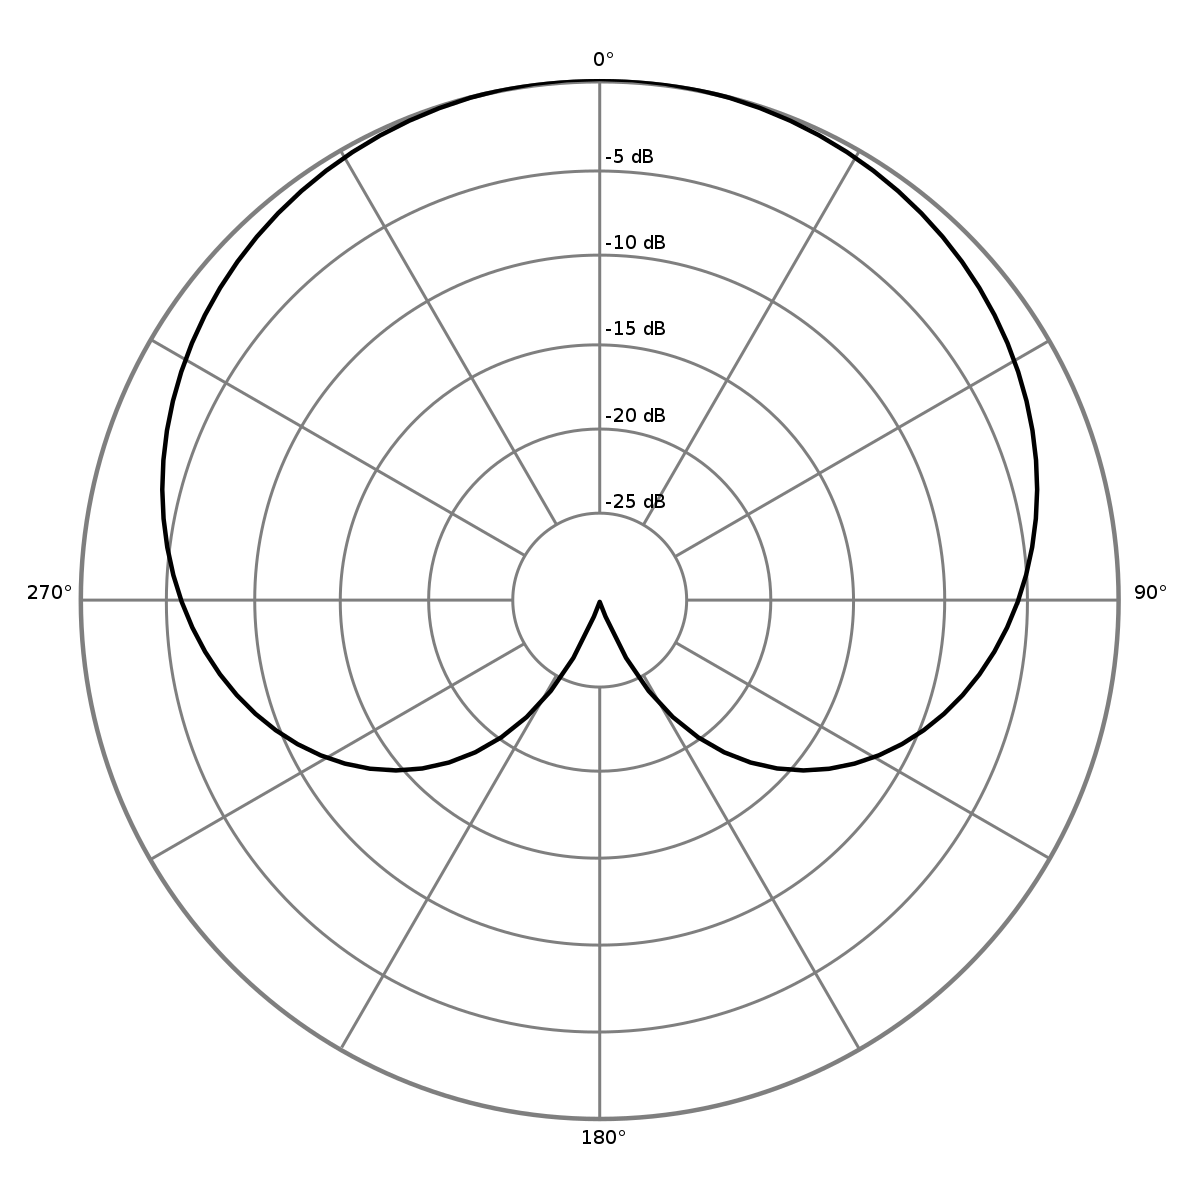
\includegraphics[width=\linewidth]{img/card.png}
  \caption{Cardioid Polar Pattern \cite{card_pic}}\label{fig:card}
\endminipage\hfill
\minipage{0.32\textwidth}
  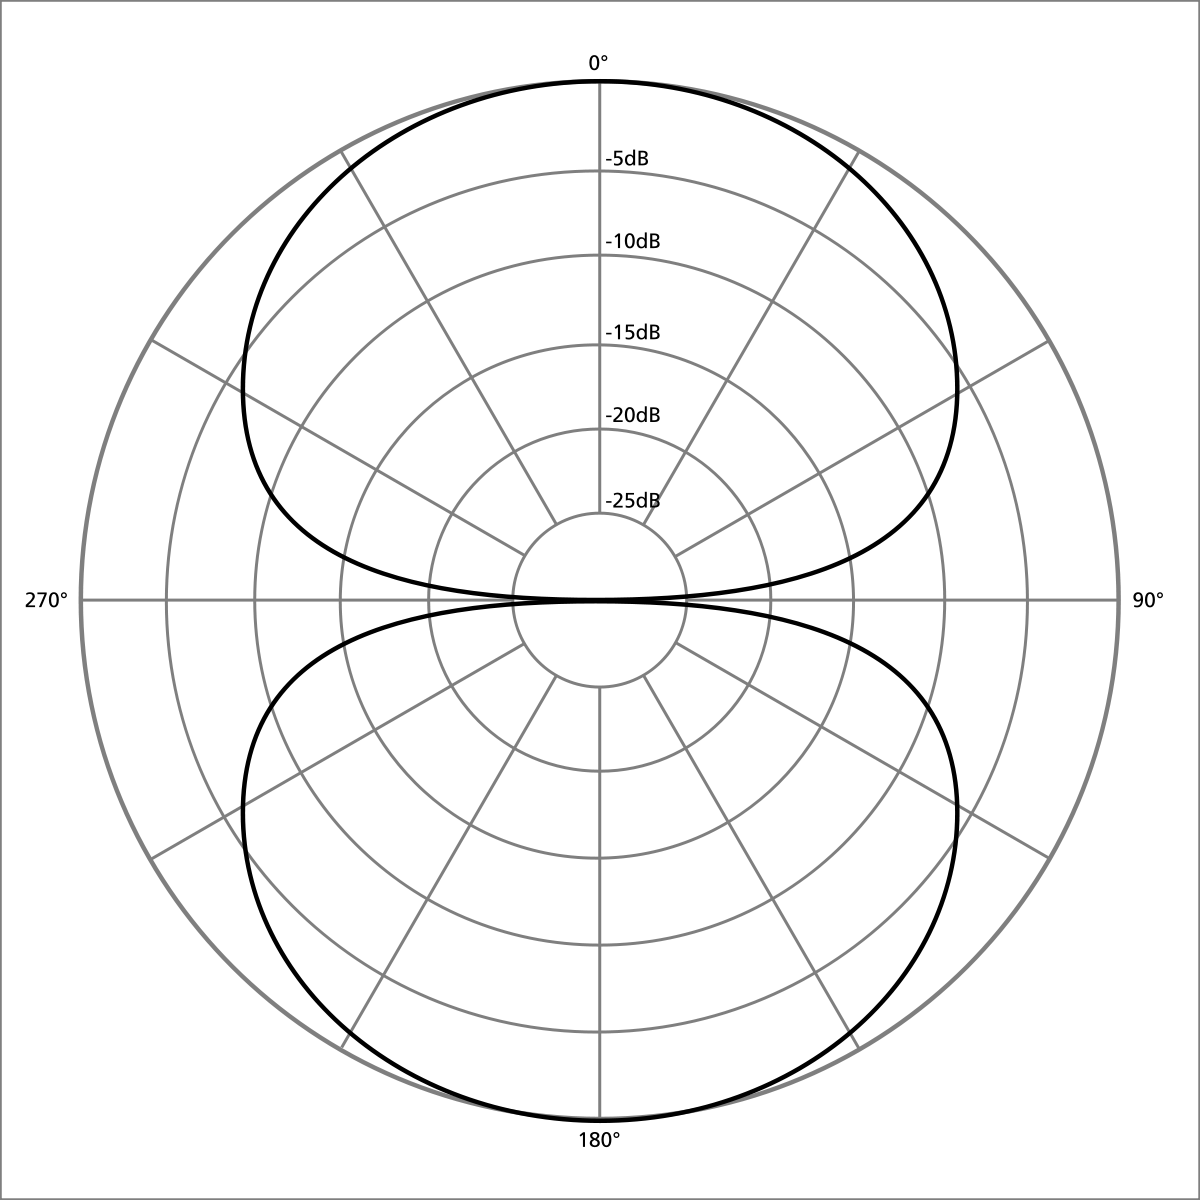
\includegraphics[width=\linewidth]{img/fig-8.png}
  \caption{Figure-8 Polar Pattern \cite{fig8_pic}}\label{fig:fig-8}
\endminipage\hfill
\minipage{0.32\textwidth}%
  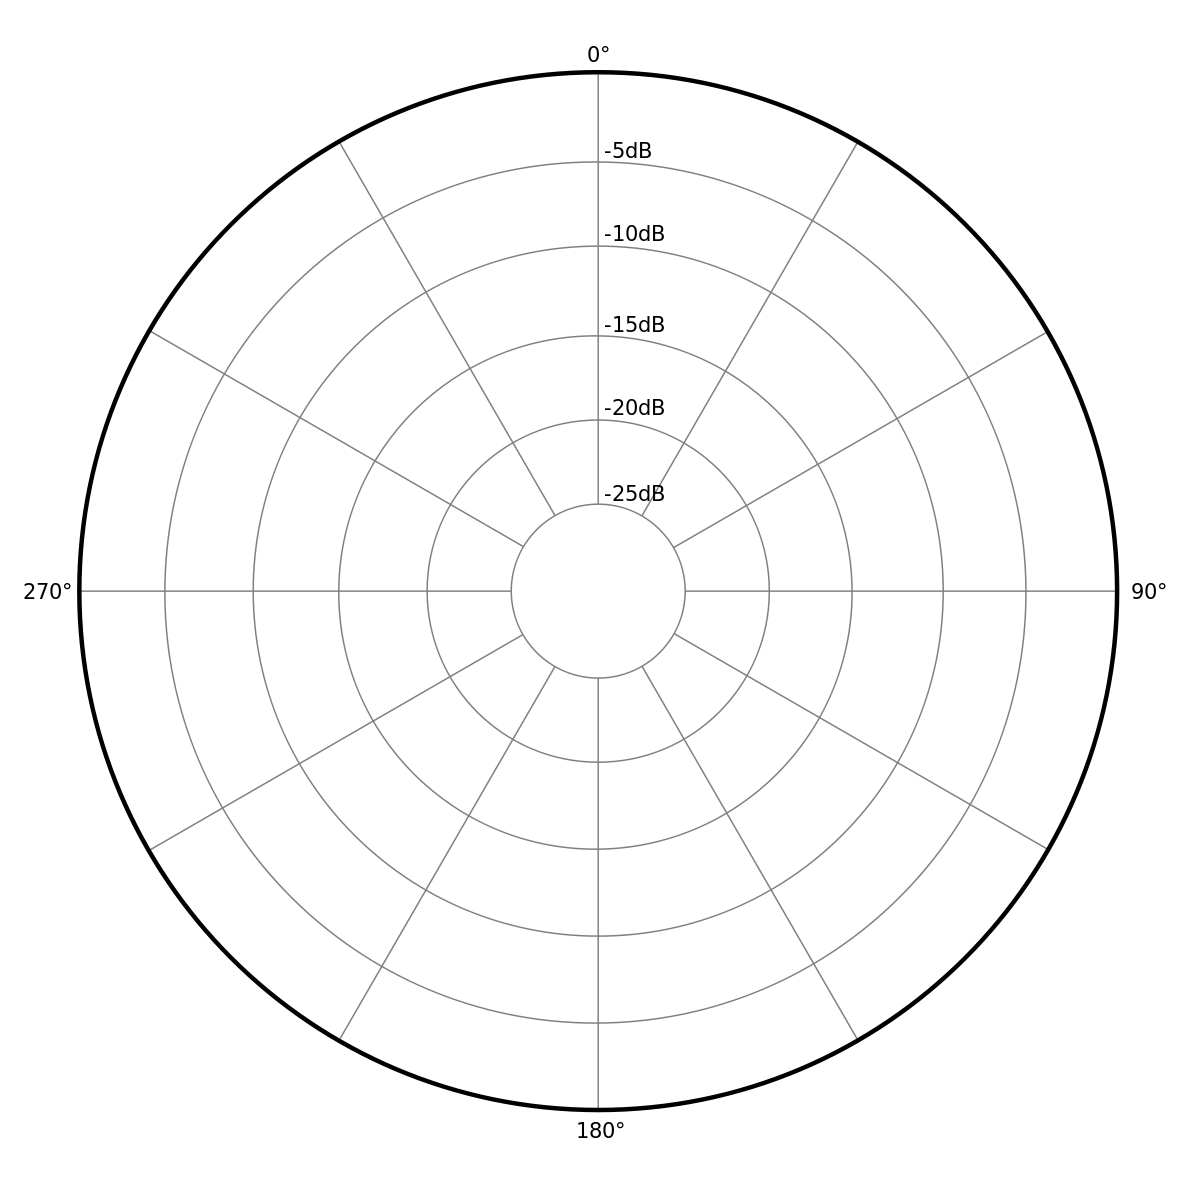
\includegraphics[width=\linewidth]{img/omni.png}
  \caption{Omni Polar Pattern \cite{omni_pic}}\label{fig:omni}
\endminipage
\end{figure}

These idealized responses show the sensitivity of different microphones to sound waves arriving from different directions. For the cardioid\footnote{Which gets it's name from it's heart-shaped response.} pattern, we see a \textit{null} at 180\textdegree and \textit{unity} response at 0\textdegree. These diagrams are seldom true in real-life, especially for high frequencies. Even for very good omni-directional microphones, eventually the capsule size becomes comparable to that of the wavelength, making the response directional. 

\textit{Off-axis coloration} refers to microphone's difference in frequency response at different directions. Most microphones can intuitively be separated into \textit{side address} or \textit{front address} microphones based on their construction. For \textit{front address} microphones, the reported frequency response will likely be based on a measurement with the capsule facing the excitation source so the response matches the ergonomic use of the microphone. Any \textit{side address} microphone, such as a cardioid condenser microphone, would perform poorly if the musician oriented the microphone backwards, resulting in a different frequency response than expected.

\textit{Proximity effect} is another term which relates to the nature of unidirectional microphones\footnote{Cardioids and figure-8 microphones fall under this category.} to exhibit a bass-boost when placed too close to the source. This is why many condenser microphones come equipped with a bass roll-off switch. The bass-boost comes from the \textit{pressure gradient} microphone. At low enough frequencies, the wavelength is vastly larger than the microphone capsule, so the difference in pressure at either side can be unnaturally large. This effect should be considered when placing musicians in relation to the microphones.

The mid-side (MS) technique previously discussed is just one of several stereo techniques that are traditionally implemented for stereo recording. While other stereo techniques such as A/B, X/Y, and ORTF also exist, these fall outside the scope of this text. The reader is referred to \cite{lipshitz1986stereo} for a lively discussion on the merits of coincident and spaced arrays for stereo reproduction. It warrants mentioning that by no means are surround-sound techniques objectively superior. In fact, there is still a lot of research being undertaken in this domain, in particular by The University of Huddersfield \cite{lee3d}. 

\textit{Spaced arrays} are a family of microphone arrays designed originally for surround sound formats. Various authors over the years have experimented and documented their configurations in order to facilitate the creation of high-quality multi-channel music for film. Figure \ref{fig:c-spaced-arrays} shows five complete spaced arrays adapted from \cite{hacihabiboglu2017perceptual} and \cite{politis2016microphone}. The diagram created is a rough approximation of these five 5.1 arrays. In addition to these five arrays, ambisonic arrays are also considered complete \textit{coincident} arrays capable of encoding surround sound formats. \cite{Immersiv9:online} also provides information about these arrays\footnote{Distances and angles might be slightly different from one reference to another. \textbf{TODO}}.

% 5.1 arrays (Fukada Tree, INA-5, Hamasaki Tree, DPA 5100, OCT-surround)
\begin{figure}[ht!]%force figure here, top, strict
\centering
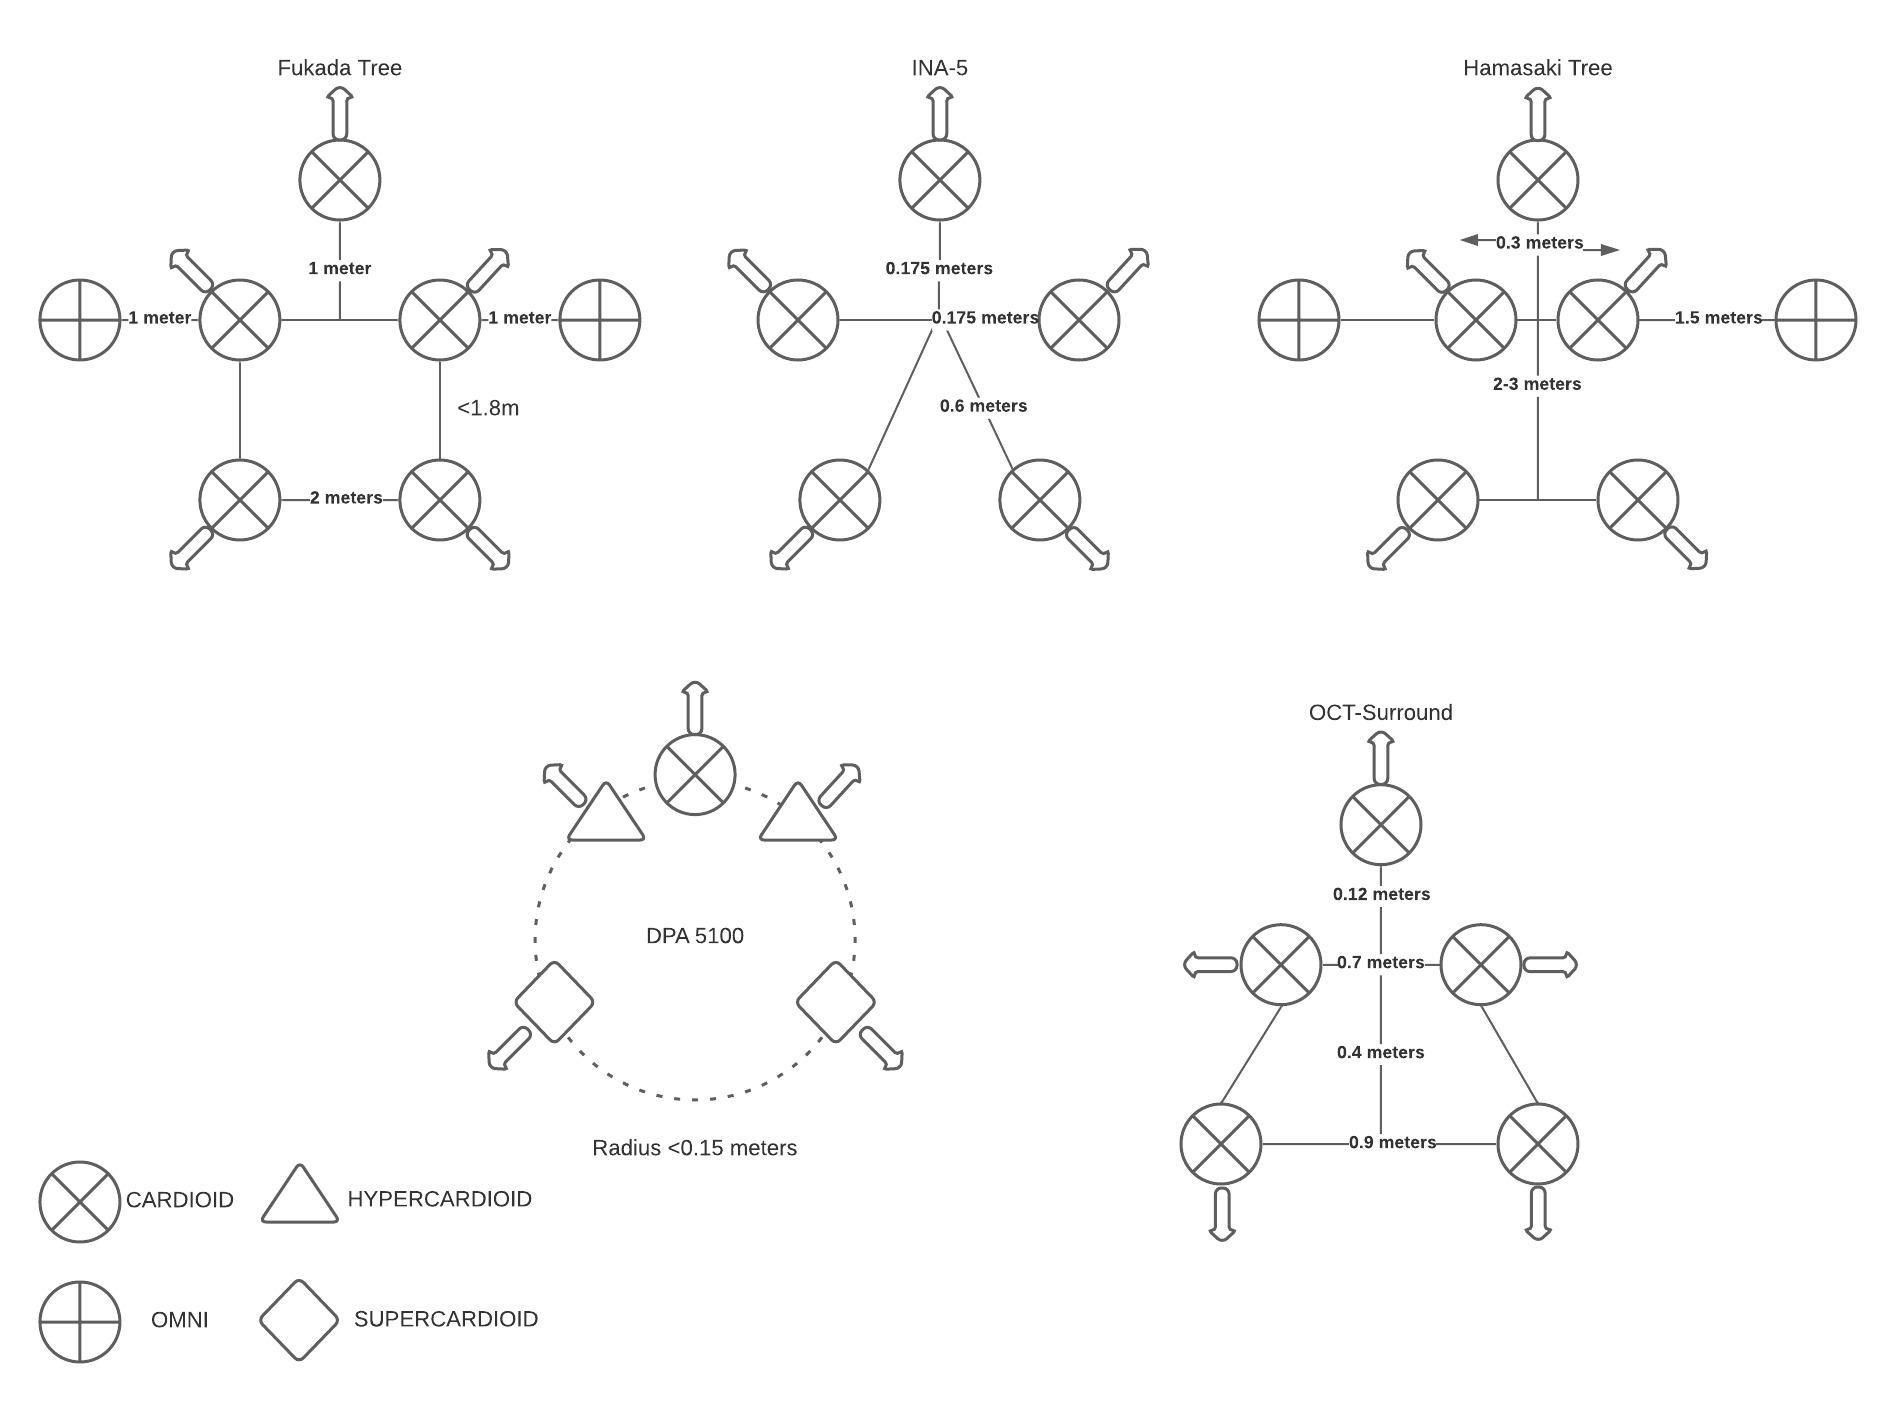
\includegraphics[width=1.0\textwidth]{img/complete-spaced-arrays.jpeg} 
%\captionsetup{justification=centering}
\caption{Complete Spaced Arrays}
\label{fig:c-spaced-arrays}

\end{figure}

\todo[inline]{The symbols I used for these drawings are not standard. Not sure if that is ok. The next list could use some detail and references.}

In addition to the five depicted arrays:
\begin{enumerate}
    \item \textbf{Fukada Tree}
    \item \textbf{INA-5} 
    \item \textbf{Hamasaki Tree}
    \item \textbf{DPA 5100}
    \item \textbf{OCT-surround}
\end{enumerate}

% Front arrays (Optimal Cardioid Triangle, Decca Tree, INA-3). Rear arrays (Hamasaki Square, IRT Cross)

A secondary technique exists for multi-channel audio recordings which involves a combination of a proximal front array and a distant rear array. In this configuration it is up to the sound engineer to decide how distantly the rear array will be placed. The decision will be based generally on the size of the space as well as how diffuse the sound is at the set distance. Front arrays include: Optimal Cardioid Triangle, Decca Tree, and INA-3. Rear arrays include: Hamasaki Square, and IRT Cross. Figure \ref{fig:fnr-arrays} shows a coarse approximation the associated arrays. The front two receivers in the rear array are summed with the side receivers from the front array in this 5.1 set-up. 

\begin{figure}[ht!]%force figure here, top, strict
\centering
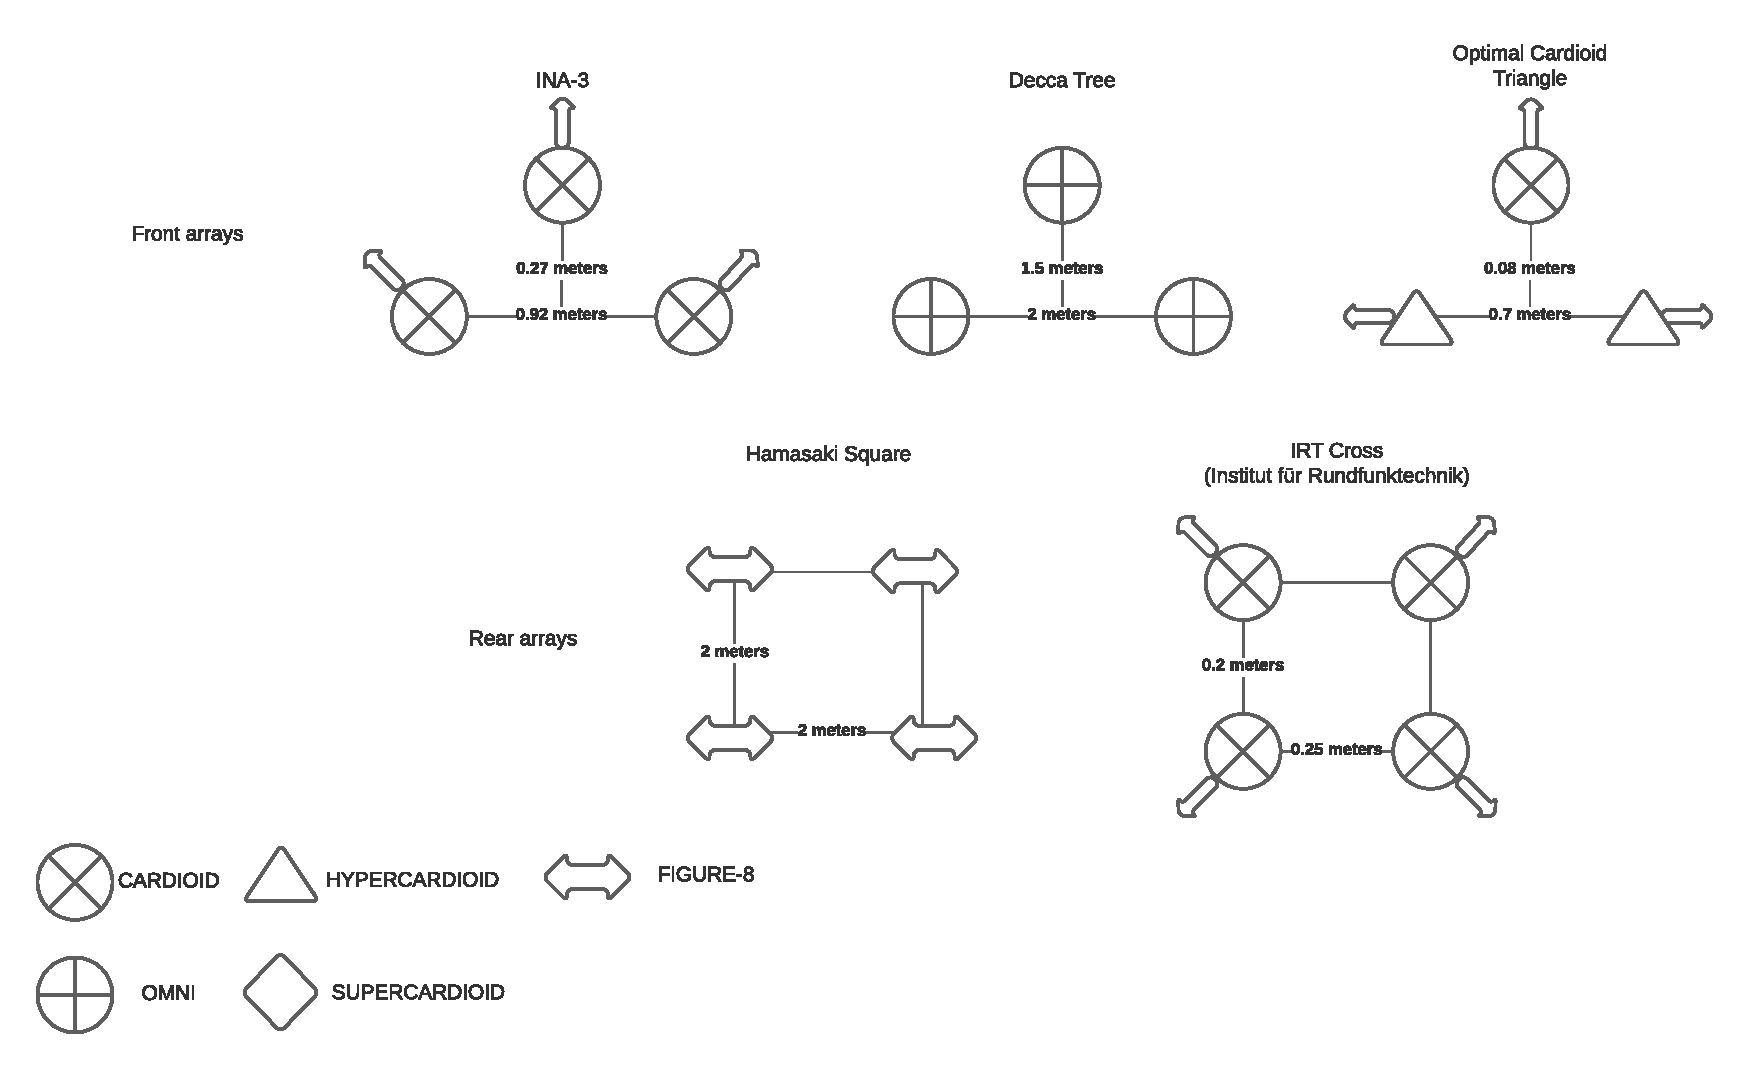
\includegraphics[width=1.0\textwidth]{img/front-n-rear-arrays.pdf} 
%\captionsetup{justification=centering}

\caption{Front and Rear Arrays}
\label{fig:fnr-arrays}
\end{figure}

\subsection{Encoding Monophonic Sources}

% The recording array from the grid mics are numbers 15+17, 18+20, and 27+30. Those mics are mixed in with the hanging ORTF pair, which moves from time to time. So that’s 6 available right now. 

The same principle of ambisonic panning, formerly introduced as a technique for creating spatial representations in music, can be extended as a recording technique for 3D audio scene construction. In this approach, rather than specifying the positions of the desired sound source trajectories, we define for the encoder the positions of the statically placed microphones used for the recording. 

For example, within our experimental concert hall at CPMC, it is possible to define a template with the location of our fixed microphone locations, used routinely for concert recording. By placing the appropriate channels in the location tracks with the corresponding panners, we can render the recordings in a multi-channel format for playback over headphones or multi-channel speaker systems. Figure \ref{fig:cpmc122-mic-grid} shows the positions of 6 microphones typically used by our house engineers for multi-track recording. An additional ORTF pair located at the center of the grid is also included in the multi-track recordings, however, the position of this pair is not perpetually fixed\footnote{According to our house engineer.}. 

\begin{figure}[h!]%force figure here, top, strict
\centering
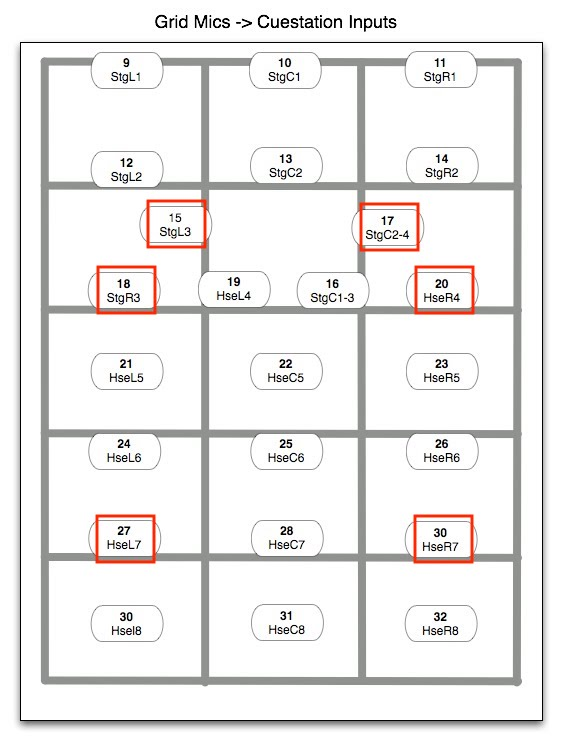
\includegraphics[width=0.5\textwidth]{img/cpmc122-mics.jpg} 
%\captionsetup{justification=centering}
\caption{CPMC122 Microphone Grid - UCSD Dept. Music}
\label{fig:cpmc122-mic-grid}

\end{figure}

A common technique implemented by recording engineers is combining multi-channel microphone arrays with fixed microphones. In the aforementioned case the 6 microphones are distant from our musicians and as a result they pick up sounds from all instruments on stage. In order to isolate sources, giving us more control in post-production, \textit{spot microphones} can be placed closer to the musicians. Ideally, the distances of all these fixed receivers are calculated in relation to the ideal listening position, both in terms of azimuth and elevation. 

\subsection{Coincident Microphone Arrays}

Of primary importance to our work is the development and optimization of coincident microphone arrays. Coincident microphone arrays come in various shape and sizes. The predominant characteristic of these devices is that proximity between sensors is minimized in order to improve localization estimations and the operating frequency \textit{virtual microphones} created by combinations of signals. There are three main types of coincident microphone arrays we were able to discern from the literature: spherical microphone arrays, studio microphone arrays, and planar microphone arrays. While most planar microphone arrays are not meant for high-quality studio recordings, we will nonetheless cover them here since many use similar operational conditions as the proposed HOA system being developed by the author. 
\subsubsection{Planar Microphone Arrays}

Planar microphone arrays are a subset of coincident microphone arrays which attempt to sample a sound-field using either a linear (one-dimensional arrays), or circular array (two-dimensional arrays). Most planar microphone arrays, although not all, fall under tha category of arrays for \textit{noise suppression}. In other words, they are not designed for multi-channel recording. Instead these devices tend to output a single audio channel that is the sum of various sensors delayed and amplified based on the desired direction(s) of sound capture. This is a technique called \textit{beamforming}, and is also applied to spherical microphone arrays.

\cite{backman2006miniature} provides some insight into planar microphone arrays and their relationship to sound-field microphones. The author in that publication relies on Micro-Electrical Mechanical Systems (MEMS) capsules for his designs, much like in our own work. Backman suggests using multiple transducers to improve signal-to-noise ratio (SNR) and improve polar pattern control over the entire audio bandwidth (20Hz-20kHz). In a second paper \cite{backman2006gradient} the author expanded upon the theoretical work proposing a 5.1 planar array based on MEMS. Unfortunately, little information was presented regarding a 3D audio capture system - the designs described were predominantly for 2D audio. 

\todo[inline]{I want to come back to these Backman papers and add more detail. There are some useful equations there. Unless they are covered more clearly in other papers.}

\cite{chen2015theory} provides a more thorough review of planar arrays. Chen's paper describes a 2D planar array designed with first order microphones which can suitably sample vertical elements of the sound-field. The benefit of planar arrays is that for certain applications, spherical arrays simply might not be possible to construct, such as in cellphone or tablet designs. One noteworthy process implemented in that publication, as well as several others, is the use of simulated responses to validate designs prior to implementation. The main problem we found with this design was the limited bandwidth which had a maximum frequency of 850Hz. For high-quality audio purposes, we seek instead to operate on the audible frequency range. Secondly, in order to sample vertical harmonics, the number of transducers had to be increased from nine, the minimum number required for 2OA\footnote{Second order ambisonics.}, to 16, which increases the cost of the final design. 

Meyer and Elko of \textit{mh acoustics}, the company responsible for the em32 Eigenmike\footnote{https://mhacoustics.com/}, described a second order augmented circular microphone in a 2008 publication \cite{meyer2008spherical}. In their paper, Meyer et al. described using a single central sensor to provide vertical control of the desired \textit{beam-pattern}. The beam-patterns are controlled by adjusting the weights in the linear combination of spatial harmonic signals (also referred to as \textit{eigenbeams} or \textit{eigenmodes}). Their design has 7 capsules "flush mounted into the top surface of a puck-like housing". There are 6 capsules along the diameter of the puck, with a radius of 3cm, along with one central capsule. This design seems suitably promising for play-back over dome-like loudspeaker systems since very few sound systems around the world have below-listener speakers. However, the design might be unsatisfactory for applications which use binaural synthesis featuring HRTFs below the listeners' ear level, since that part of the sound-field would not be properly reconstructed. Two other details stand out about the design:

\begin{enumerate}
    \item The microphones are described as pointing upwards rather than outwards. Mounting them on the side of the puck would have likely improved the performance of the array. 
    \item The author's never specify what capsules are used and there is little information regarding how to recreate the experiment.
\end{enumerate}

There are also two metrics mentioned by Meyer et al. we should discuss Directivity Index (DI) and White Noise Gain (WNG). The DI is the difference in \textit{decibels} between the sound pressure level (SPL) in a given direction and the average SPL from an omni-directional source \cite{LONG201439}:

$$
\mathrm{D}(\theta, \phi)=\mathrm{L}_{\mathrm{p}}(\theta, \phi)-\overline{\mathrm{L}}_{\mathrm{p}}
$$
where \\
    $\mathrm{D}(\theta, \phi)=$ directivity index $($ gain $)$ for a given direction $(\mathrm{dB})$ \\
    $\mathrm{L}_{\mathrm{p}}(\theta, \phi)=$ sound pressure level for a given direction $(\mathrm{dB})$ \\
    $\overline{\mathrm{L}}_{\mathrm{p}}=$ sound pressure level averaged over all angels $(\mathrm{dB})$ \\
    $(\theta, \phi)=$ some specified direction.

\todo[inline]{Make sure you are consistent with phi and theta in your code. phi should be azi. and theta should be elev. Also, the formatting here is inconsistent. Consider using d}

% \begin{equation}
% \begin{array}{l}
% W=S \cdot \frac{1}{\sqrt{2}} \\
% X=S \cdot \cos \theta \cos \phi \\
% Y=S \cdot \sin \theta \cos \phi \\
% Z=S \cdot \sin \phi
% \end{array}
% \end{equation}

WNG is a quality metric of beamforming algorithms. It is defined as the beaformer's ability to suppress spatialy uncorrelated noise. Note that self-noise and external white noise may be statistically indistinguishable, so WNG constraints should consider self-noise as well. Mismatch between sensor characteristics and position errors can also result in spatially white noise \cite{mabande2009design}. 

\todo[inline]{middlicott 5 channel array, ambi, circular}

% According to the authors, directional microphones, are less well-matched than omni-directional microphones. Matching capsules is important for good sound-field sampling. 

% As the author suggests, most authors today are less interested in horizontal only audio capture, and even less so in systems which only sample the sound-field in 1D - likely because surround sound has encouraged the creation of material with 2D qualities. Extending WFS to a 2D representation yields a similar representation to that generated by VBAP \cite{smith2019spatial}. 
% Planar microphone arrays have nonetheless become increasingly popular as systems for direction-of-arrival (DOA) estimation and subsequent beamforming operations. In these systems, the linear microphone array is used to estimate the DOA of a signal using statistical analysis of the signals. Then, a beamforing operation can be performed on these same signals to generate a highly directive microphone pattern \textit{pointing} at specified location. This can be used, for example, to isolate and improve the quality of recording for a speaking person within a noisy environment. The same principle has also been applied to circular and spherical arrays. 

\subsubsection{Spherical Microphone Arrays}

Spherical microphone arrays (SMA) are particularly interesting to us because they represent a simple way of capturing spatial sound both in a studio setting and in nature. In contrast to other recording techniques in which musicians' coordinates need to be defined in order to create a adequate sound-field, spherical microphone arrays inherently capture this information into what are called \textit{A-format} recordings. These recordings are then encoded into the spherical domain for reproduction over an arbitrary loudspeaker configuration or binaural system. 

SMAs can further be separated into three types of arrays: rigid, hollow, and tiered. Tiered arrays constitute arrays in which various radii are superimposed in order to capture different regions of interest of the sound-field \cite{dabin2015design}. In general, these systems have gotten less attention due to the difficulty of integrating these models with camera systems. Rigid and hollow models are more popular, and corresponding mathematical formulations exist for both. At their names suggest, a rigid spherical microphone array has no cavities exposed to the outside of the array, while the hollow designs do have open spaces over which sound may propagate.

% In general, rigid microphone arrays have gotten the most attention from the commercial sector, because of the elegance of their complimentary design with multi-camera systems, however, hollow arrays have also been implemented commercially in audio-only designs, targeted towards audio engineers who are not interested in producing video content. 

Over the years several authors, including the present author, have proposed spherical microphone arrays, generally, tough not always, with the intention of recording and reproducing ambisonic signals. The degree to which these designs have been documented and made open to the public varies from author to author. The following pages describe some attempts made over the years to create open-source spherical microphone arrays. In the commercial sector, there are also designs by companies such as: Sennheiser, Zoom, and Zylia. 

\paragraph{Modular Spherical Microphone Array (MSMA)}

Gonzáles et al. \cite{gonzalez2018modular} published in 2018 a design the defined as "modular" given the systems ability to change radius on-the-fly. Actually, their design can also be considered a multi-tiered since in certain configurations it can have more than one operating radius. The project site can be found \href{https://www.appropedia.org/Modular_Spherical_Microphone_Array}{here} (accessed: Feb. 2021). In the cited publication the authors compared the performance of their design in three configurations: small radius, large radius, and mixed-radius. 

Some of the key features of this design, in addition to the modularity aspect of the microphone, is the use of FOSS for the Computer Assisted Design (CAD)\footnote{The authors used OpenSCAD, which is distinct from other systems in that the user program the design using lines of code, rather than manual manipulations.} and MicroElectrical Mechanical Systems (MEMS) microphones in lieu of Electret Condenser Microphones (ECM). Unfortunately, the code used to generate the CAD models does not seem to be accessible but the files for manufacturing the Printed Circuit Boards (PCB) and the rendered 3D designs, for 3D printing, can be downloaded. 

In order to validate their designs, the authors used a simulation approach which they compared to the ideal characteristics of spherical harmonics. The "Spherical Array Processing" library by Archontis Politis, publicly downloadable from Github, and explained in his doctoral dissertation, was used for this assesment. The spatial correlation is given by the following equation: 

\begin{equation}
R_{\left|S^{s i m}\right|,\left|S^{S H}\right|}=\frac{\left\langle S^{s i m}, S^{S H}\right\rangle}{\left\|S^{s i m}\right\| \cdot\left\|S^{S H}\right\|}
\end{equation}

The top part of the fraction involves taking the dot product of the simulated and ideal spherical harmonics. The bottom part involves taking the norm of each vector and then calculating their product. These are all classic operations of linear algebra. 

Unfortunately, these simulations can only give us an approximation of the performance of this system. Ideally, the authors would have also measured the response of the microphone in anechoic conditions. However, the design is promising in that the parts used for its manufacturing can be printed with low-cost 3D printers. This modular spherical microphone array (MSMA) also features MEMS capsules, making it more affordable to reproduce than other designs. Unfortunately, the 19 capsules require a rather costly interface in order to record the signals. MEMS microphones with internal ADCs might provide a cheaper alternative than the proposed analog MEMS devices. 

\paragraph{Higher Order Spherical Microphone Array (HOSMA)}

TH Köln\footnote{University of Applied Sciences is an institute of higher education located in Cologne, Germany.} has published several papers describing the development of a rigid Spherical Microphone Array (SMA). In (moschner-2020-open-source-mic-array.pdf) the authors describe their latest efforts to create a 7th Order Ambisonic (7OA) microphone with a total of 64 capsules. As the authors noted, spherical harmonic processing in VST plug-ins is limited to 64 channels (ie. SPARTA, IEM).  There are currently no 7OA microphones on the market, the highest order commercial system is the Eigenmike by mh acoustics which is of 4th order. 

Simiarly to Gonzáles et al. this microphone system has an inner sphere to which various tubes are attached, however, in the case of the design by Moschner et al. the 64 channels are all comprised of ECM capsules instead of MEMS microphones. This microphone design uses the same capsules as the commercial FOA microphone by Sennheiser: Ambeo VR Mic. The CAD modeling is done in Blender and the analysis is done using the SOFiA toolbox\footnote{\href{https://github.com/AudioGroupCologne/hosma}{Link to HOSMA repository} (accessed: Feb 26, 2021)}. 

%% sampling grids

% fliege grid
% http://www.personal.soton.ac.uk/jf1w07/nodes/nodes.html

% fliege grid and t-designs
% http://research.spa.aalto.fi/projects/sht-lib/sht.html

\subsubsection{Studio Microphone Arrays}
%This section describes some studio coincident microphone arrays. 

These are all studio techniques in which microphones are placed as close together as physically possible. 

Native B-format array, double MS, double MSZ, etc.

\subsection{Arrays in Series}

A modern type of sound capture technique has recently been developed and is the subject of great interest for spatial audio researchers. The technique, predominantly employed under the basis of ambisonic rendering, involves capturing multiple sound-fields simultaneously using an \textit{array of arrays}. In other words, a recording engineer positions a grid of multiple spaced microphone arrays in such a way that the \textit{acoustic boundaries} of adjacent arrays overlap each other. 

The goal of this capture technique is to allow, within a digital representation, six degrees of freedom (6DoF), or, \textit{translational} movement, in addition to the standard rotational control. Figure \ref{fig:6DoF} shows these translational transformations where yaw, pitch, and roll correspond to rotational transformations. 

\begin{figure}[h!]%force figure here, top, strict
\centering
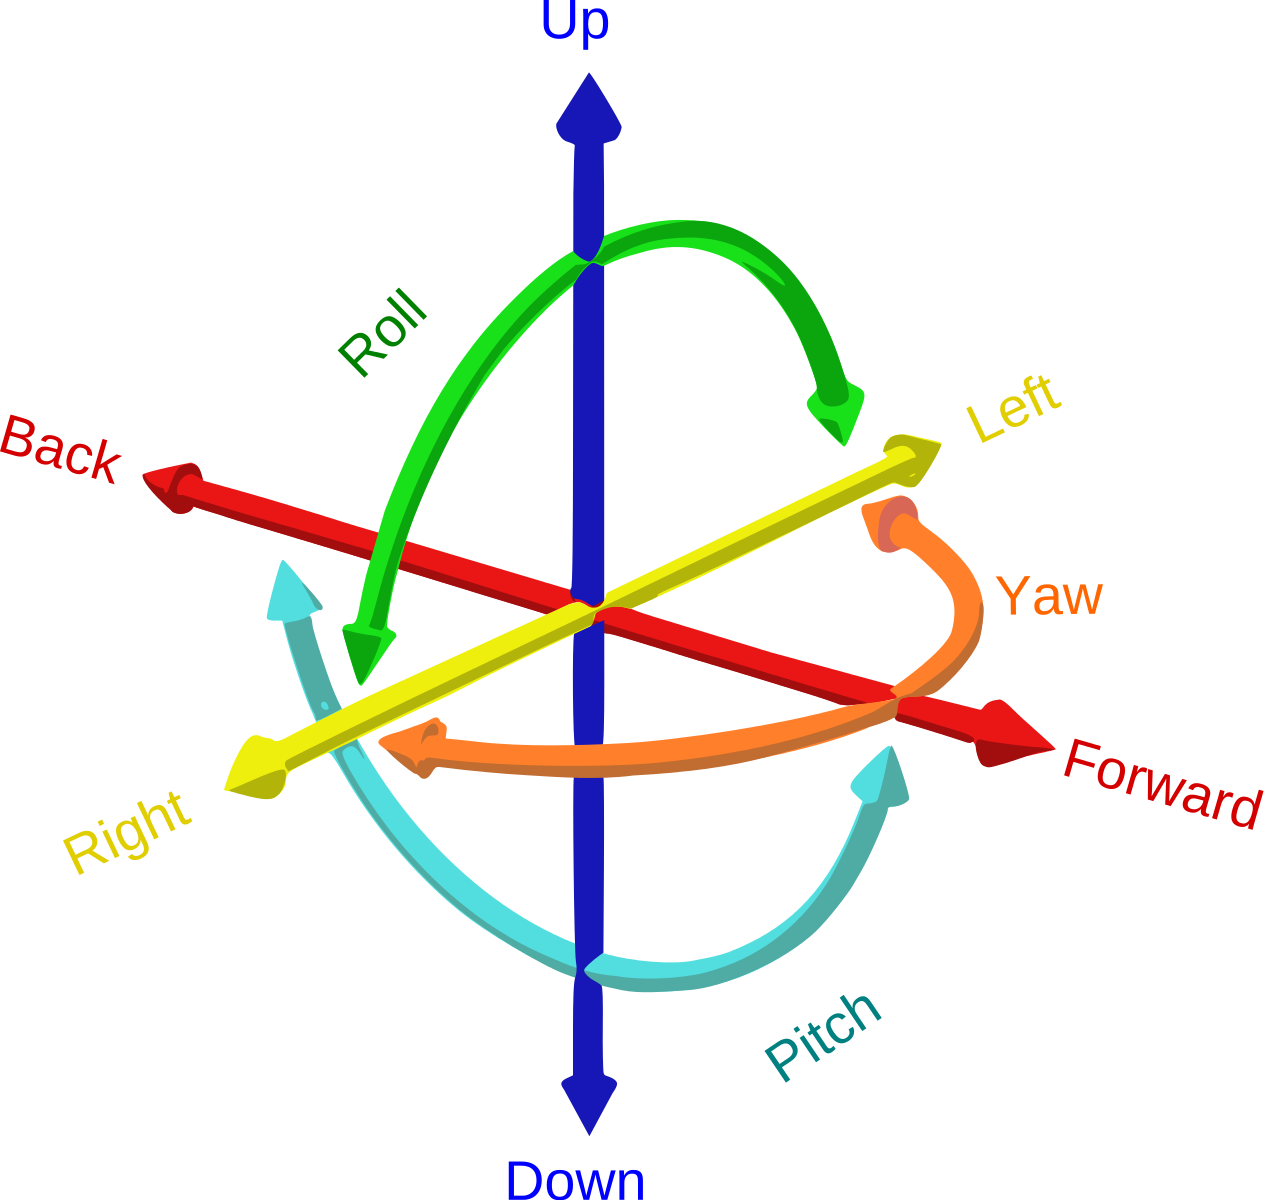
\includegraphics[width=0.5\textwidth]{img/6DOF.svg.png} 
%\captionsetup{justification=centering}
\label{fig:6DoF}
\caption{6DoF - wikimedia commons}
\end{figure}

\section{Open Tools for Spatial Audio Capture}

\todo[inline]{what about video editors? Blender? DaVinci Resolve? }

A number of authors have described the development of Free and Open Source Hardware (FOSH) for the capture of real sound-fields for either asynchronous or synchronous transmission. The majority of these designs fall under the category of spherical microphone arrays although other projects exist which discuss alternative geometries for spatial audio capture. While many publications have been presented wherein the authors describe the creation of such systems, few have actually sought to provide full documentation detailing the process undertaken to realize the entire system. 

A common problem with these designs for musicians seeking to enter the world of sound-field recording is the costly price-point of some of the Bills of Materials (BoMs) suggested by the engineers. In order to swap parts, the musician would need to know about electronics specifications and how to modify Computer Assisted Design (CAD) files in order to create his or her own systems.

\section{Contemporary Spatial Audio Reproduction Techniques} \label{sec:contemp_audio_reproduction}

In the previous section we talked extensively about the artists and engineers who have shaped the way we think and talk about spatial sound. The various sections to follow will provide a look into some of the state-of-the-art research regarding spatial audio solutions and the: composers, institutions and practices, which are pushing us to further our understanding and curiosity. 

\subsection{Amplitude Panners}
\label{subsec:amplitude panner}

\todo[inline]{VBAP, DBAP, other panners, octo, quad, etc. kapralos-2008-virtual-aud-sys-mit.pdf see 4.2.2 amplitude panning. Zirkonium. }

Out of the various iterations of "x-based systems"\footnote{Such as VBAP, DBAP, etc.} the most prominent and well-regarded is called \textit{Vector Based Amplitude Panning} (VBAP). In his 1997 paper \cite{pulkki1997virtual} Pulkii describes how trigonometric operations can be used to position a sound in any position in 3D space. The idea behind VBAP is to create \textit{phantom images} between sources giving listeners the illusion that sounds emanate from any arbitrary position between 2 or more speakers. Pulkii, the inventor of VBAP, from Helsinki, Finland, writes in regards to the difference between this method and ambisonic panning\footnote{Ambisonic panning does not use spherical microphones but encodes arbitrary audio sources for ambisonic reproduction.}: "the gain factor calculation in the VBAP method equals that of the Ambisonics in an orthogonal\footnote{Regular loudspeaker layouts.} loudspeaker placement". 

The key difference between VBAP and ambisonic panning, is that VBAP generalizes calculates the gains for any irregular layout, making it more flexible in some regards. Ambisonics, however, can be encoded without knowing anything about the reproduction system, while in VBAP we need speaker positions in order to calculate the signal gains. 

While these two systems might seem remarkably similar, experiments have suggested that there exist statistically significant perceptual differences for both reproduction methods (Marentakis 2014). VBAP has gained much popularity among composers due to it's simplicity and elegance. A MAX/MSP collection of externals were developed by Pulkii in 2000 to allow electronic musicians to experiment with the system making it fairly accessible. It should be noted that as with many other spatialization methods it relies heavily on a great number of speakers for successful immersion. 

% \subsection{Modeling}
% \subsubsection{Wave-Based Modeling}

% Wave-based modeling involves solving the wave equation, also known as the \textit{Helmholtz-Kirchoff} equation, to create a Room Impulse Response (RIR) that models a particular sound-field. 

\subsection{Object Based Audio}
\label{subsec:oba}

Object Based Audio (OBA) is a format agnostic method, much like ambisonics, in which audio objects carry metadata which are used by the \textit{renderer} to successfully reproduce each sound source \cite{coleman2018audio}. Some of the parameters included in the metadata of each audio object include: level, position, radius, and spread\cite{fug2014design}. In contrast to ambisonics, in which the sound-field might be pre-rendered, OBA requires real-time rendering of objects within a scene. The benefit of this method is that the listener gains control of the "mix". Using OBA the listener can, for example, adjust the balance between dialog and background sounds - a feature which highly desirable since a preponderance of background sounds can sometimes reduce speech intelligibility beyond comprehension. There are several software platforms which support OBA, here we will only cover a few and focus particularly on systems related to computer-music.

\paragraph{MPEG-H}

Among the various technologies used to create OBA, the MPEG-H\footnote{The Moving Picture Experts Group (MPEG) is an alliance of working groups of ISO (International Organization for Standardization) and IEC (International Electrotechnical Commission) that sets standards for media coding, including compression coding of audio, video, graphics and genomic data, and transmission and file formats for various applications.} COder/DECoder (CODEC) has become the most popular in commercial settings. Herre describes OBA in \cite{herre2015mpeg}:

\begin{quote}
    More recently, the merits of object-based representation of a sound scene have been embraced by sound producers, e.g. to convey sound effects like the fly-over of a plane or space ship. Audio objects are signals that are to be reproduced as to originate from a specific target location that is specified by associated side information. In contrast to channel signals, the actual placement of audio objects can vary over time and is not necessarily pre-defined during the sound production process but by rendering it to the target loudspeaker setup at the time of reproduction. This may also include user interactivity.
\end{quote}

VBAP and OBA are closely related as reproduction methods. In fact, OBA typically uses VBAP in order to render the sound objects. In addition, the MPEG-H framework also includes the possibility of streaming HOA and discrete channels data (typically used in surround sound formats) in order to synthesize a hybrid format. Furthermore, the standard counts with a consistent perceptually motivated compression system used to lower the amount of data required for accurate spatial reproduction. One can sign-up to receive some authoring software for MPEG-H via the  \href{https://www.iis.fraunhofer.de/en/ff/amm/dl/software/mas.html}{Fraunhofer website}. Some other projects have embraced the Opus CODEC for compression in streaming solutions requiring spatial audio\footnote{One such project is \href{Earshot}{https://github.com/EnvelopSound/Earshot} by Envelop.}.

\paragraph{SpatGRIS}

Recently, the Groupe de Recherche en Immersion Spatiale (GRIS) at Université de Montréal published a self-proclaimed OBA authoring system called \textit{SpatGRIS/ServerGRIS}. Previously, SpatGRIS was used in conjunction with the Zirkonium software\footnote{https://zkm.de/en/about-the-zkm/organization/hertz-lab/software/zirkonium} from ZKM. Today, ServerGRIS serves as a standalone spatialization system which can be used in conjunction with ServerGRIS to spatialize sounds in dome-like environments via VBAP. SpatGRIS has two modes, one in which it performs the spatialization itself, and one in which it sends OSC data to ServerGRIS. SpatGRIS also works with DAWs which route audio via JackRouter to ServerGRIS to perform the gain adjustments. In this sense, one can consider the GRIS system as an OBA format, since each audio channel has an associated data track defining its spatial properties.

The software's user interface makes use of \href{https://en.wikipedia.org/wiki/Cocoa_(API)}{Cocoa} which makes it solely compatible with macOS\footnote{Not compatible with Catalina (10.15) as of Jan 29, 2021.}. One of the benefits of SpatGRIS/ServerGRIS over the VBAP external for Pd, for example, is that the software provides a binaural renderer which allows the user to audition their multi-channel work over headphones. Unfortunately, there does not seem to be a way to dynamically rotate the sound-field as with HOA, so the binaural rendering will be static. The software is also more dynamic than the Pd VBAP system with regards to re-routing of audio signals in different environments, and, automating trajectories in a DAW is far more comfortable than doing so in Pd, which requires the user specifying coordinates using a text editor. 

Ledoux, one of the authors of the GRIS software, describes the benefits of OBA:

\begin{quote}
    This object-based audio approach has the advantage of dissociating sound source’s localisation from the loudspeakers position and allows pre-spatialized music to be portable from one dome to another, regardless of the amount of loudspeakers and their relative position. \cite{ledoux2018immersive}
\end{quote}

\paragraph{Commerical Solutions}

In addition to the MPEG-H system, Dolby Atmos and DTS:X also offer OBA solutions. Both companies have a long tradition of driving the market and have proposed standards for multi-channel film production over the years. Mac and PC version of the Dolby software can be found \href{https://developer.dolby.com/tools-media/production-tools/dolby-atmos-mastering-suite-updates/downloads/#!}{here}. The DTS-X creator suite can be purchased \href{https://dts.com/production-tools/#creator-suite}{here}. DTS-X also counts with a video player which can playback ambisonics. The reader is referred to \href{https://www.videolan.org/vlc/releases/3.0.0.html}{VLC} for a FOSS video player, which can reproduce ambisonics and even has binaural support. 

\paragraph{SpatDIF}

One final project that might interesting to the reader is SpatDIF which is short for \textit{Spatial Sound Description Interchange Format} \cite{peters2012spatdif}. The project as it stands is mostly defunct now but the Pd externals can still be \href{https://www.zhdk.ch/en/research/icst}{found online} at the ICST website from ZHDK\footnote{Zürcher Hochschule der Künste or "Zurich University of the Arts". Zurich is the largest city in Switzerland.}. The SpatDIF project is now integrated into the ZKM\footnote{ZKM Center for Art and Media Karlsruhe is in Germany.} \href{https://zkm.de/en/about-the-zkm/organization/hertz-lab/software/zirkonium}{Zirkonium} software. 

The Zirkonium software is actually built with Pd but the GUI is only OSx compatible. SpatDIF aimed to store the trajectories of sound objects as XML files that could be read by Pd in real-time. The user could use VBAP or Ambisonics to render the sound objects in their scene. It should be noted that SpatDIF never explicitly calls itself an OBA system, but we believe it could still be categorized as such because each sound has an associated scene description which is used by a renderer at a later stage for reproduction in an arbitrary loudspeaker layout. 

One of the main drawbacks we should point out with OBA is that the number of sound sources will change the number of channels to the stored. This will also be a consideration at the rendering stage. The larger the number of sources, the more computationally expensive it will be to render the sources in real-time. In contrast, ambisonic allows us to represent an arbitrarily large number of sound sources in a limited number of channels with varying quality based on the ambisonic order \cite{scaini2020wavelet}. Scaini provides another definition of OBA in his recently published thesis on wavelet-based spatial-audio framework\footnote{Based on spherical wavelets.}: 

\begin{quote}
    In object based formats the role of encoding and decoding is essentially reversed with respect to the channel based formats. There is no spatial encoding, and the task of generating the gains for each speaker is given to the decoding stage, where a panning law is used at playback time to convert the object metadata into gains. Here the panning law does not define the format, and it is possible to use different panning laws for the same object based format, providing that the panning law ‘understands’ the object metadata.
\end{quote}

\todo[inline]{soundscape renderer?}

%https://github.com/mgeier/spatdifrenderer
%https://sourceforge.net/projects/omprisma/

\subsection{Wave Field Synthesis}
\label{subsec:wfs}

%https://github.com/GameOfLife/WFSCollider

Whilst less commonly seen or talked about, \textit{Wave Field Synthesis} (WFS) is another area of interest for acousticians and composers. WFS attempts to capture a wavefront and reproduce it at a later stage. A good case scenario for this is the simulation of a live concert. A wall of microphones is placed ten meters from the band and, at a later point, a wall of speakers is used to play back the recorded audio. A new audience could in theory listen to this reproduction and be transported to the event. The audience members could even walk around the "dance floor" and experience the rich spatial detail as if they were really there. WFS is a powerful spatial technique but entirely context dependent. It is often not desirable for situations in which sound arriving from all directions need to be captured. WFS also costly, as proper capture and reproduction takes dozens of microphones and speakers, making it inaccessible for most consumers.

\subsection{Higher Order Ambisonics}
\label{subsec:ambi}

Ambisonics is a full-sphere capture and reproduction method popular among spatial audio enthusiasts. A resurgence in interest, as with any of the aforementioned methods, can be attributed to the growth of mixed reality\footnote{MR is a term used for augmented reality experiences in which digital objects can be interacted with.}, augmented reality (AR) and virtual reality (VR) systems. Ambisonics has become one of the de facto spatial audio reproduction methods for simple VR experiences, especially 360\textdegree \ video. Large tech companies have adopted it as a standard in immersive video content.  

Ambisonic signals can be created by panning traditional monophonic recordings or by capturing them via an ambisonic microphone. A tetrahedral microphone, the simplest ambisonic microphone, captures First Order Ambisonic (FOA) A-format\footnote{A-format audio is ambisonic audio from a mic prior to encoding.} signals which can be used to reproduce 360 degrees of spatial audio with tolerable quality. 

The theory and application of ambisonic heavily relies of the assumption that the playback system is composed of a spherical array of speakers which situates the listener at the origin. The tetrahedron shape, or three-sided pyramid, is the lowest geometric approximation of a sphere. This shape is thus chosen for FOA capture. Higher approximations result in a higher number of channels and better spatial quality at the cost of more data to be handled and stored. The assembly and calibration of Higher Order Ambisonic (HOA) microphones remains a laborious. As a result, HOA panning of mono signals is used more commonly.

One of the major limitations of ambisonics recordings captured with HOA microphones over other techniques, such as OBA, is the fact that the listener is confined to the geometric position in which the recording was taken in (or synthesized for). In VR, AR and MR, users generally are not satisfied with being stationary - even if they can turn and tilt their heads. These recordings work suitably well for viewers experiencing 360\textdegree \ videos, but if users want to traverse a digital playground, they will not be able to do so convincingly. It could therefore be said that whilst ambisonic can provide a good ambience layer for these experiences, it relies heavily on other strategies for full immersive experiences. Recent research efforts have focused on the interpolation between sound-fields, such that users can move around freely between various ambisonic recordings taken in proximity to each other. 

\todo[inline]{Need to add citation to that last sentence. Also a bit repetitive.}

\subsubsection{Mathematical Formulation}

\subsubsection{Decoding Strategies}

Decoding of ambisonic signals refers to the process of taking B-format spherical harmonics and linearly combining these to produce speaker signals. As we have mentioned before, ambisonics is best suited for regular loudspeaker layouts. Regular speaker layouts in the spherical domain include those modeled after the five \textit{platonic solids}. These include the tetrahedon (4 faces), cube (6 faces), octahedron (8 faces), dodecahedron (12 faces), and icosahedron (20 faces). Each of the faces of these \textit{convex regular polyhedra} is represented by a speaker in our layout. 

Unfortunately, placing listeners at the center of such geometries, which would correspond to the ideal listening location, is often difficult - since this requires speakers below and above the listener. In very sophisticated listening environments, an acoustically transparent grid is often employed which allows speakers to be placed below the listener. An additional layer of complexity arises from determining the ideal circumference of the listening area. We ideally need to find a balance between the size of the reproduction area, and the proximity to any individual speaker. 

A lot of research has been undertaken in the domain of ambisonic decoding for irregular layouts \cite{heller2008my}. The general process used to decode ambisonic signals, involves computing the real-valued spherical harmonics for the speaker positions ($\mathbf{L}$) and subsequently calculating the decoding matrix by finding the inverse of this matrix ($\mathbf{D}$). The resultant matrix $D$ is multiplied with the matrix of ambisonic signals $\mathbf{B}$ yielding the speaker feeds ($\mathbf{G}$). The size of the decoding matrix becomes $L$ x $(N + 1)^2$, where $L$ is the number of loudspeakers and $N$, as always, is the \textit{ambisonic order}. 

Heller \cite{heller2008my} provides a magnificent introduction to decoder design. One of the points that Heller raises is that some poor decoding designs, such as ones where all frequencies are decoded exactly the same, produce \textit{comb-filtering}\footnote{Phase errors caused by two complex signals being played simultaneously with a small delay between them.}. Instead, notable improvements can be made if the user performs \textit{velocity decoding} at low frequencies, and \textit{energy decoding} at high frequencies. \textit{Near-Field Compensation} (NFC) can also be applied for sources that one wishes be perceived as being inside the listening area. 

Three additional factors Heller mentions which may affect decoder quality include: 

\begin{enumerate}
    \item Room acoustics.
    \item Accuracy of speaker positioning and matching\footnote{The frequency and phase response measured at the center of the array should be identical.}.
    \item Timing errors in multi-channel \textit{Digital to Analog Converters} (DACs).
\end{enumerate}

While these criteria were developed for multi-channel decoders, the same principles can be applied to binaural decoders \cite{gorzel2019efficient}. When dealing with binaural reproduction, however, we must consider headphone equalization if we wish to achieve perfectly transparent playback. The term used for headphone equalization filters is generally \textit{Headphone Related Transfer Functions} (HpRTF). These filters are designed to compensate for the frequency and phase response of headphones, ideally modifying them so they are completely flat and linear.

\paragraph{Defining the Problem: Decoding Ambisonic Signals}

According to Heller \cite{heller2008my}, a decoder must meet three criteria for proper reproduction: 

\begin{enumerate}
    \item Velocity and energy vector directions are the same at least up to 4kHz, and substantially unchanged with frequency. 
    \item At low frequencies, the magnitude of the velocity vector is near unity for all reproduced azimuths. 
    \item At mid/high frequencies the energy vector magnitude is substantially maximized across as large a part of the sound-stage as possible.  
\end{enumerate}

In the next few paragraphs we will cover how each of these criteria can be satisfied. Certain formulae will be introduced in order to frame the problem and help understand what is meant by velocity and energy vectors.

\begin{equation}
P=\sum_{i=1}^{n} G_{i}
\end{equation}

$P$ is used to designate the pressure, and $G_{i}$ is used to designate the possibly complex gains from the source to the $i$-th loudspeaker. 

\begin{equation}
E=\sum_{i=1}^{n}\left(G_{i} G_{i}^{*}\right)
\end{equation}

$E$ is used to denote the total energy gain. $G_{i}^{*}$ is the complex conjugate of $G_{i}$. This means the real part of the complex number returned by the FFT will be the same, but the imaginary part will have opposite sign\footnote{For example $a + bi$ becomes $a - bi$ where $i$ is the imaginary number and $a$ and $b$ are real numbers.}

The \textit{velocity localization vector} and \textit{energy localization vectors} $\mathbf{r_{V}}$ and $\mathbf{r_{E}}$ can be decomposed into their component parts. The magnitude and the direction of the velocity vector is subsequently given by:

\begin{equation}
r_{V} \hat{\mathbf{r}_{\mathbf{V}}}=\frac{1}{P} \operatorname{Re} \sum_{i=1}^{n} G_{i} \hat{\mathbf{u}}_{\mathbf{i}}
\end{equation}

In this case $r_{V}$ corresponds to the magnitude and $\hat{\mathbf{r}_{\mathbf{V}}}$ corresponds to the direction of the velocity vector. These equations assume the measurements are done at the center of the array with $n$ loudspeakers. $\hat{\mathbf{u}}_{\mathbf{i}}$ corresponds to the unit length vector in the direction of the loudspeaker.



\paragraph{Computing the Low-Frequency Decoding Matrix} 



\paragraph{Computing the High-Frequency Decoding Matrix} 



\paragraph{Merging the LF and HF Matrices} 



% Gorzel paper, Politis AmbiJS paper, todo.

\todo[inline]{beam forming, constellation system for adaptive room acoustics (reverb)?}

\subsection{Binaural Synthesis}
\label{subsec:bin-synth}

\todo[inline]{XTC subsubsection}

\cite{cuevas20193d} provides an extensive literature review on the subject of \textit{binaural spatialization}. In this particular text by Cuevas, one of the most comprehensive writings on binaural synthesis, the authors describe the steps undertaken for each part of the signal chain. Figure \ref{fig:3dti-chain} shows a diagram of the implementation. 

For the \textit{free-field} modeling, an anechoic system based on BIRs/HRIRs is implemented, following:

\todo[inline]{barycentric interpolation?}

\begin{enumerate}
    \item Distance-dependent attenuation (inverse square law or acoustic power law), this step also includes far-field distance simulation modeling air impedance (distance-dependent low-pass filtering).
    \item HRIR obtained using \textit{barycentric interpolation} and are ITDs removed to dynamically adjust for different head sizes.
    \item HRIR convolution.
    \item ITD is computed and added to the signals.
    \item ILD correction for \textit{near-field} sources.
    \item Directional features for hearing aids added(if any).
\end{enumerate}

For the \textit{diffuse-field} modeling, a non-anechoic system based on BRIRs\footnote{Note that BRIRs are not taken in free-field, so these contain reflections.} is implemented as follows:

\begin{enumerate}
    \item Independent distance-dependent attenuation to control the \textit{direct-to-reverberant ratio} (DRR). 
    \item Sources are encoded into 1st Order Ambisonic (FOA).
    \item These channels are convolved with encoded versions of the BRIRs, which have been processed to remove any direct sound.
\end{enumerate}

\begin{figure}[ht!]%force figure here, top, strict
\centering
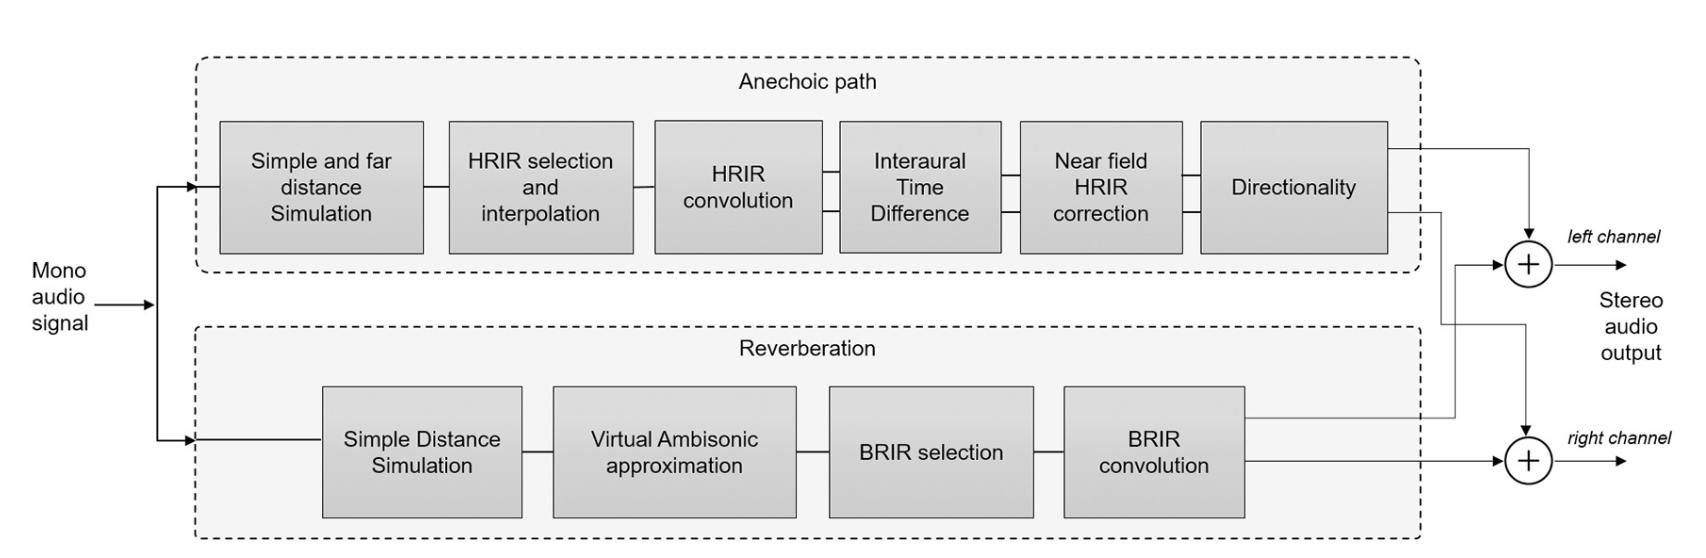
\includegraphics[width=1.0\textwidth]{img/3dti-chain.png} 
%\captionsetup{justification=centering}
\caption{3DTI Toolkit Binaural Structure \cite{cuevas20193d}}
\label{fig:3dti-chain}
\end{figure}

% \subsection{Spherical Speaker Arrays}

\section{Open Tools for Spatial Audio Reproduction}

\todo[inline]{DAWs and VSTs, not CPU mus languages. video players VLC.}

\cite{nettingsmeier2008ambi} provides us with a good description of the processes required to adequately set up an ambisonic playback system at home. We are interested in these particular solution not just because of the robustness of the method, but also because it was designed using all open source software. The benefit of open source software is that it is generally free, and, as a result, it lowers the overall cost of having to mount systems such as the one described. Naturally, a system like this one would still remain far more prohibitive than ambisonics over binaural synthesis within a WebVR experience - for example - but the comparison is really like comparing apples to oranges, WebVR, or any other commercial VR solution, is far from being able to achieve complete multi-modal\footnote{By multi-modal we mean: stimulating more than one sense. "Ideally" the experience would trick all five senses.} immersion.

In the aforementioned publication the author employs a hexagonal horizontal-only speaker set-up, however, it should be noted, the biggest benefit of ambisonics in the context of creating spatial music is the proliferation of binaural decoders for the method which allow one to forego speaker systems entirely\footnote{The quality of the final mix will be dependent on the quality of the binaural decoder.}. What this means is that if a composer is interested in creating music for HDLAs, they need not have access to a sophisticated loudspeaker system - they only need a pair of headphones and computer. In certain contexts, however, it is useful to have multi-channel systems operational and calibrated (for a spatial music class, for example). 

In such a case, where a "real" loudspeaker set-up is required Nettingsmeier, provides us with a good description of the associated steps required to calibrate such a system. Summarily, the steps in that paper are:

\begin{enumerate}
    \item Get all the gear you need, checking that: drivers for interfaces are supported by OS\footnote{You will need a decent amount of RAM. The higher order ambisonics the more RAM will be needed.}.
    \item Organize the number of speakers you have available in the desired layout (in his case a hexagon). 
    \item Measure the distances and angles from the center position and adjust speakers so the vertices of the ideal polygon (or polyhedron) match the mathematical model.  
    \item With the measured angles and distances, create a decoder using the AmbDec by Fons Adriansen\footnote{For Linux only. See ambi-X, IEM Plug-in Suite, or ATK for other systems.}.
    \item Use Aliki and Digital Room Correction (DRC) software to create six correction filters\footnote{This requires a good quality omni mic, such as the umik-1 by miniDSP (used in our work). Alternatively one can borrow a Earthworks M30, or similar measurement microphone from their University.}.
    \item Use an RMS meter to "level match" all your speakers. For this step and the last the center of the "rig" should be the reference point. 
    \item Listen and modify based on your preference. You can change your mind and build a new decoder, or remove speakers if you want. 
\end{enumerate}

\begin{figure}[ht]%force figure here, loosely
\centering
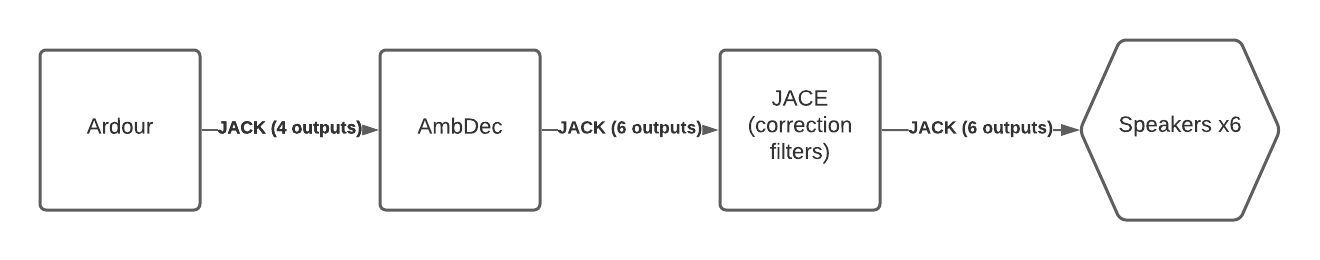
\includegraphics[width=1.0\textwidth]{img/nettingsmeier-extra-frontal.png} 
%\captionsetup{justification=centering}
\caption{Nettingsmeier Ambi System}
\label{fig:extra-frontal}
\end{figure}

Figure \ref{fig:extra-frontal} shows the signal flow for Nettingsmeier's simple home ambisonic system. We chose to generalize the signal flow since the choice of hardware is mostly irrelevant, and we seek to understand a framework that is modular and flexible. The correction filters mentioned are created to counter the imperfect frequency reproduction of the speakers as well as the effects of room acoustics. The \href{https://jackaudio.org/}{Jack software} is used to connect different associated audio algorithms for the final reproduction. It should be noted that this solution was presented over ten years ago, since then other software packages have been released which allow for more streamlined FOS\footnote{Free and open source.} ambisonics. 


\section{Conclusion}